\section{Characterizing \bc Traffic}\label{sec:charachterzing_bc}

%\par In this section, we investigate the characteristic of Bitcoin traffic, try to identify Bitcoin traffic in unencrypted and encrypted traffics. First we analyze the block propagation delay in Bitcoin network. Then, we use the results to come up with a scheme to correlate the client's traffic with a known baseline for Bitcoin blockchains in order to detect the Bitcoin usage in client traffic.

In this section, we demonstrate the unique features of \bc traffic. We will show that such unique traffic patterns of \bc  makes it reliably distinguishable from other protocols even despite encryption and mixture with background traffic. 
We will use our characterization  to 
design classifiers for \bc in the following sections.
All of our experiments in this section follow the 
 experimental setup and datasets described in Section~\ref{sec:exp-dataset}. 

\begin{table*}
\caption{Number and percentage of each message in a 31 days Bitcoin traffic in compact block relaying}
\centering
\begin{tabular}{|c|c|c|c|} \hline
Message & Packets per minute & Proportion  & Average packet size\\ \hline
\code{inv} & 173.17 & 27.240\% & 791.87\\ \hline
\code{getdata} & 13.16 & 2.070\%  & 700.33\\ \hline
\code{block} & 0.94 & 0.330 \%  & 772.74\\ \hline
\code{sendcmpct} & 1.60 & 0.253\%  & 782.88\\ \hline
\code{cmpctblock} & 2.02 & 0.319\% & 789.21 \\ \hline
\code{getblocktxn} & 0.02 & 0.003 \%  & 367.67\\ \hline
\code{blocktxn} & 0.77 & 0.121\%  & 777.16\\ \hline
\code{tx} & 277.72 & 43.688\%  & 790.00\\ \hline
\end{tabular}
\label{table:msg_proportion}
\end{table*}


\begin{figure*}[h]
\centering
\begin{subfigure}{0.24\linewidth}
\centering
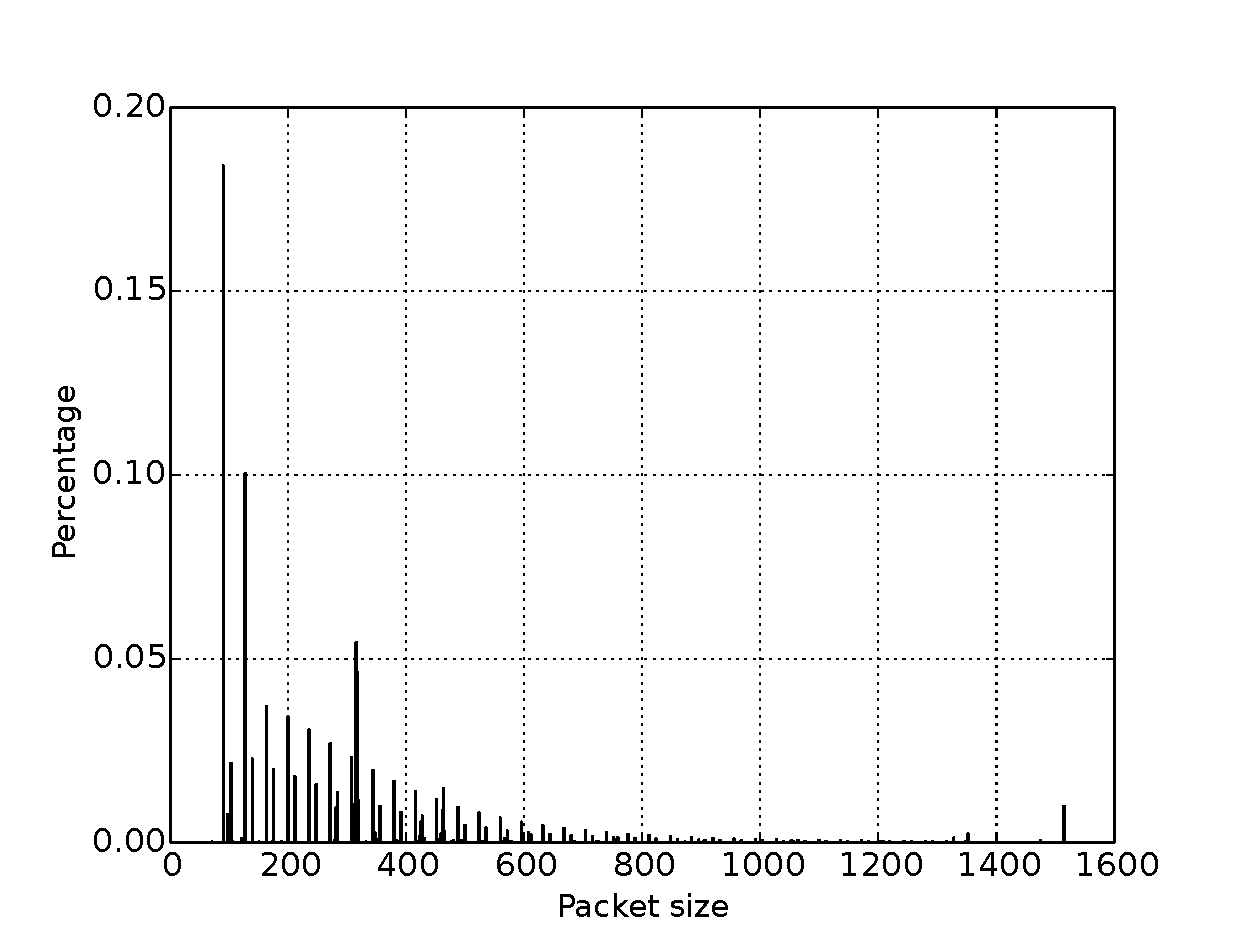
\includegraphics[width=\linewidth]{image/inv_pktsizes.eps}
\caption{\code{inv}}
\label{fig:inv_pktsizes}
\end{subfigure}
\begin{subfigure}{0.24\linewidth}
\centering
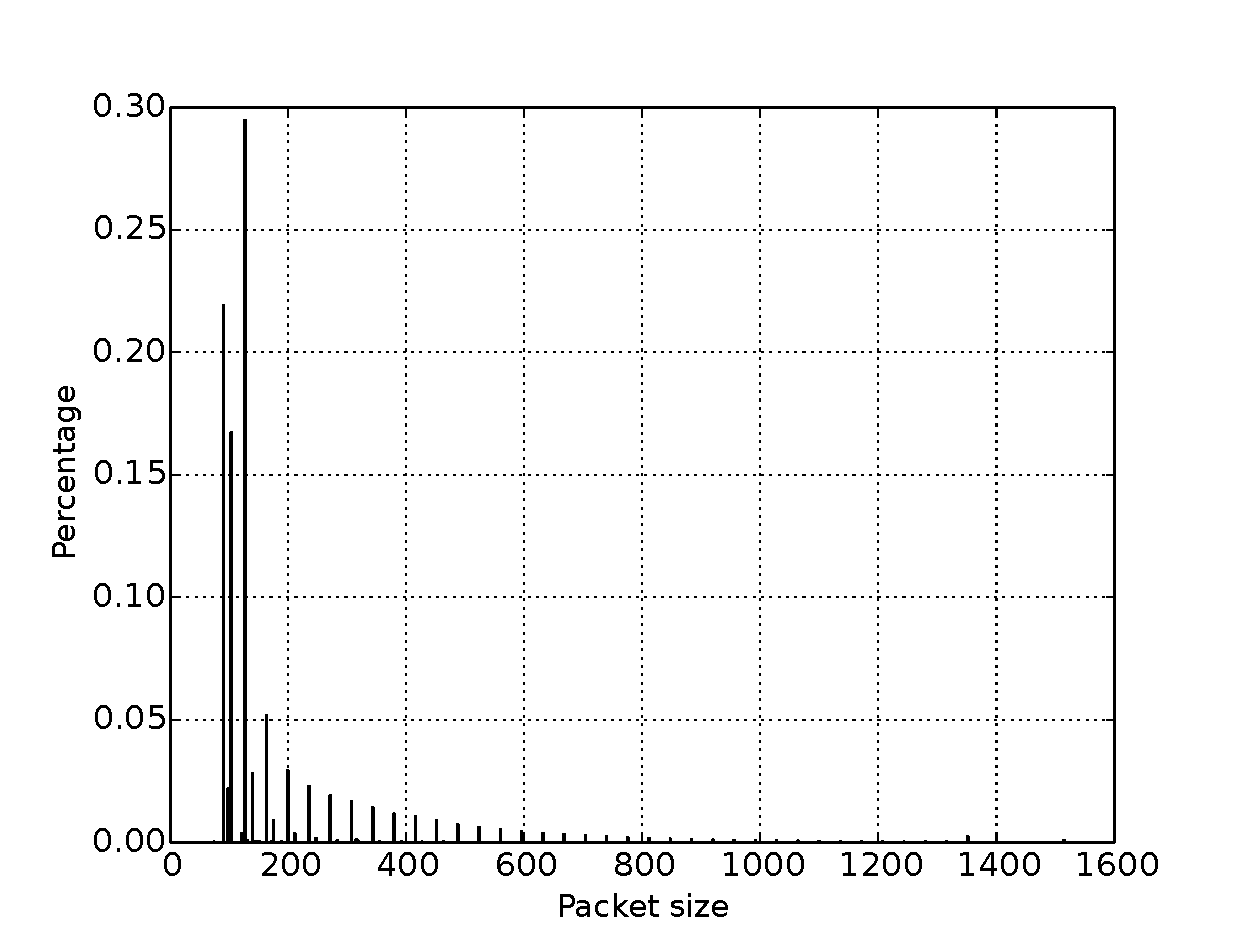
\includegraphics[width=\linewidth]{image/getdata_pktsizes.eps}
\caption{\code{getdata}}
\label{fig:getdata_pktsizes}
\end{subfigure}
\begin{subfigure}{0.24\linewidth}
\centering
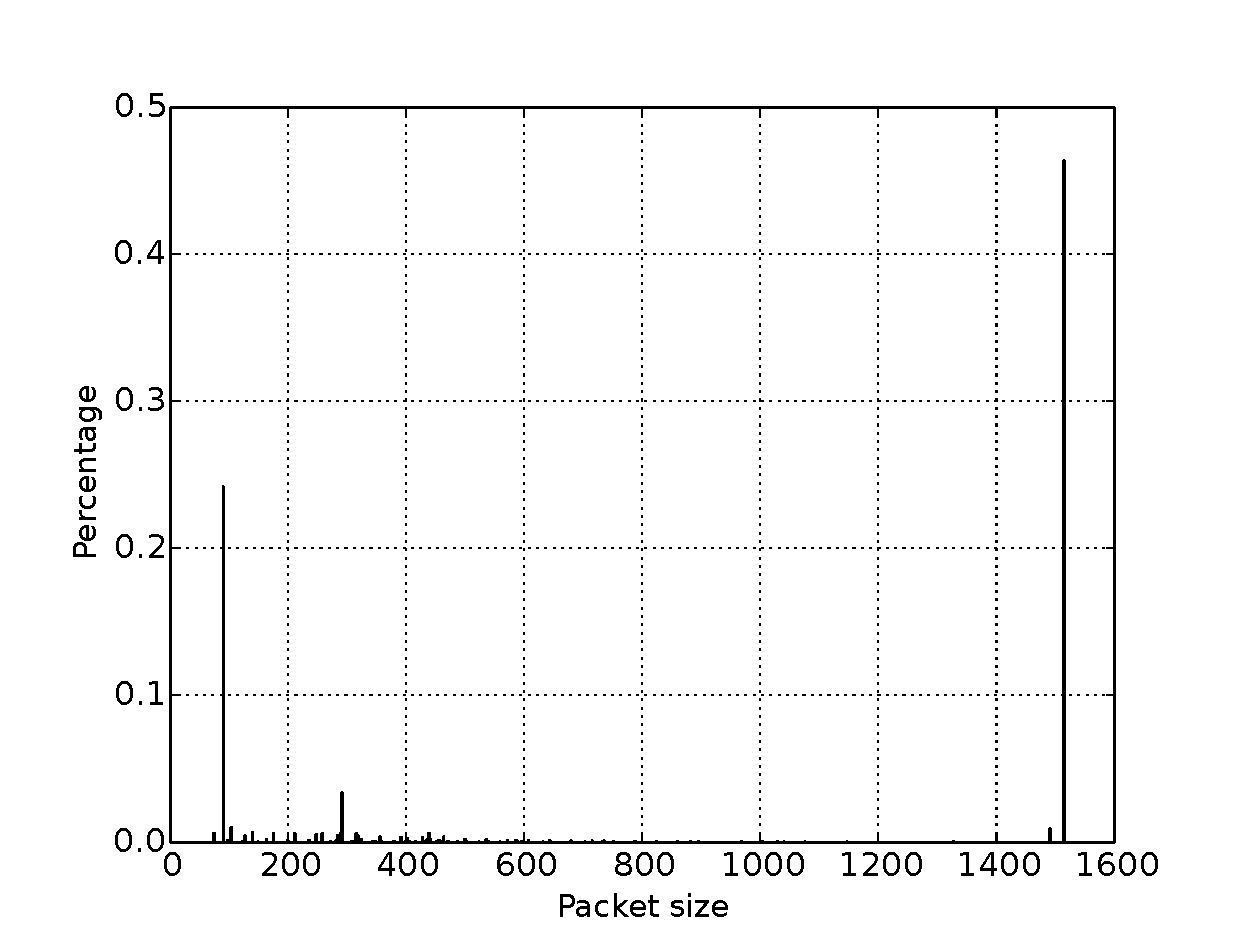
\includegraphics[width=\linewidth]{image/block_pktsizes.eps}
\caption{\code{block}}
\label{fig:block_pktsizes}
\end{subfigure}
\begin{subfigure}{0.24\linewidth}
\centering
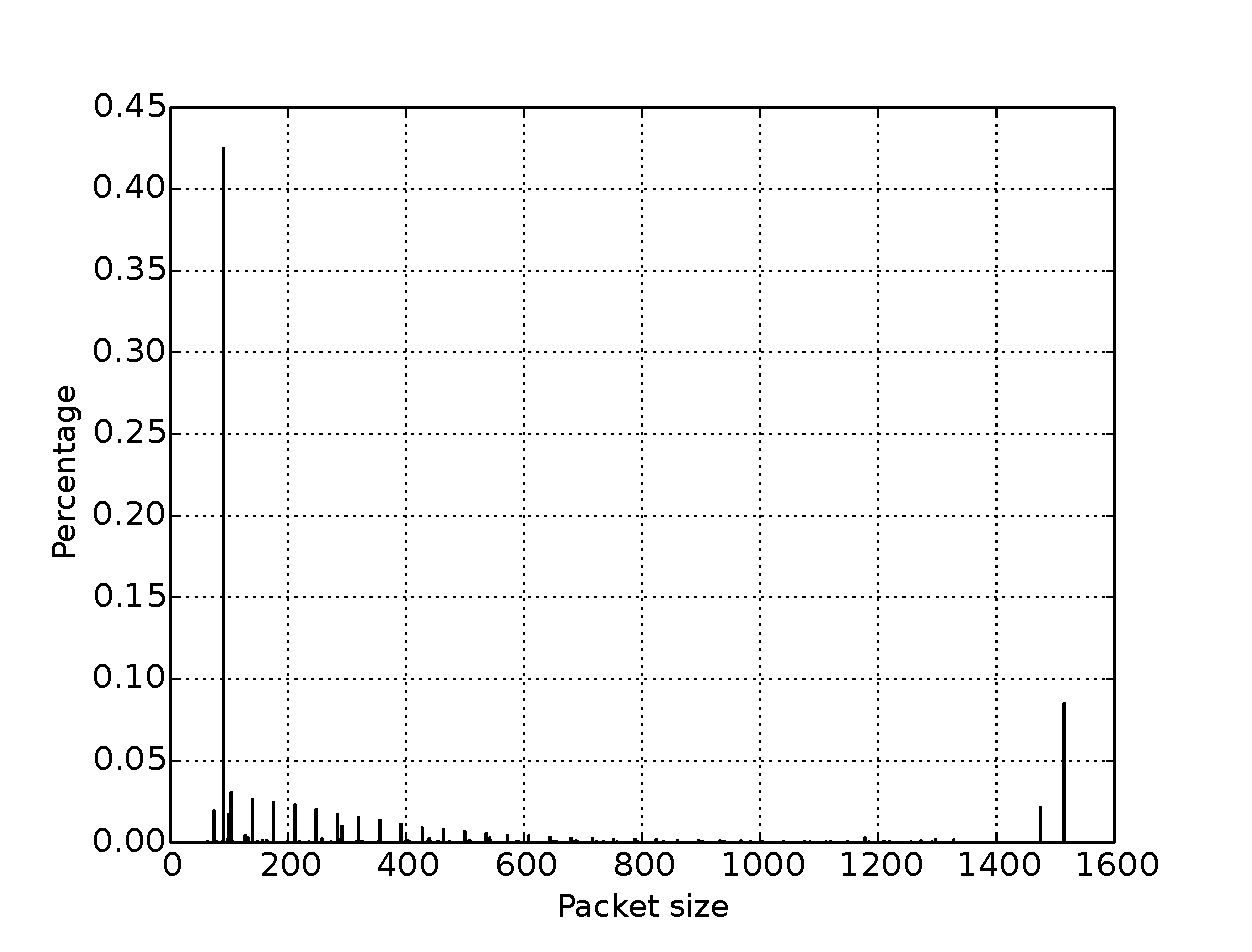
\includegraphics[width=\linewidth]{image/sendcmpct_pktsizes.eps}
\caption{\code{sendcmpct}}
\label{fig:sendcmpct_pktsizes}
\end{subfigure}
\begin{subfigure}{0.24\linewidth}
\centering
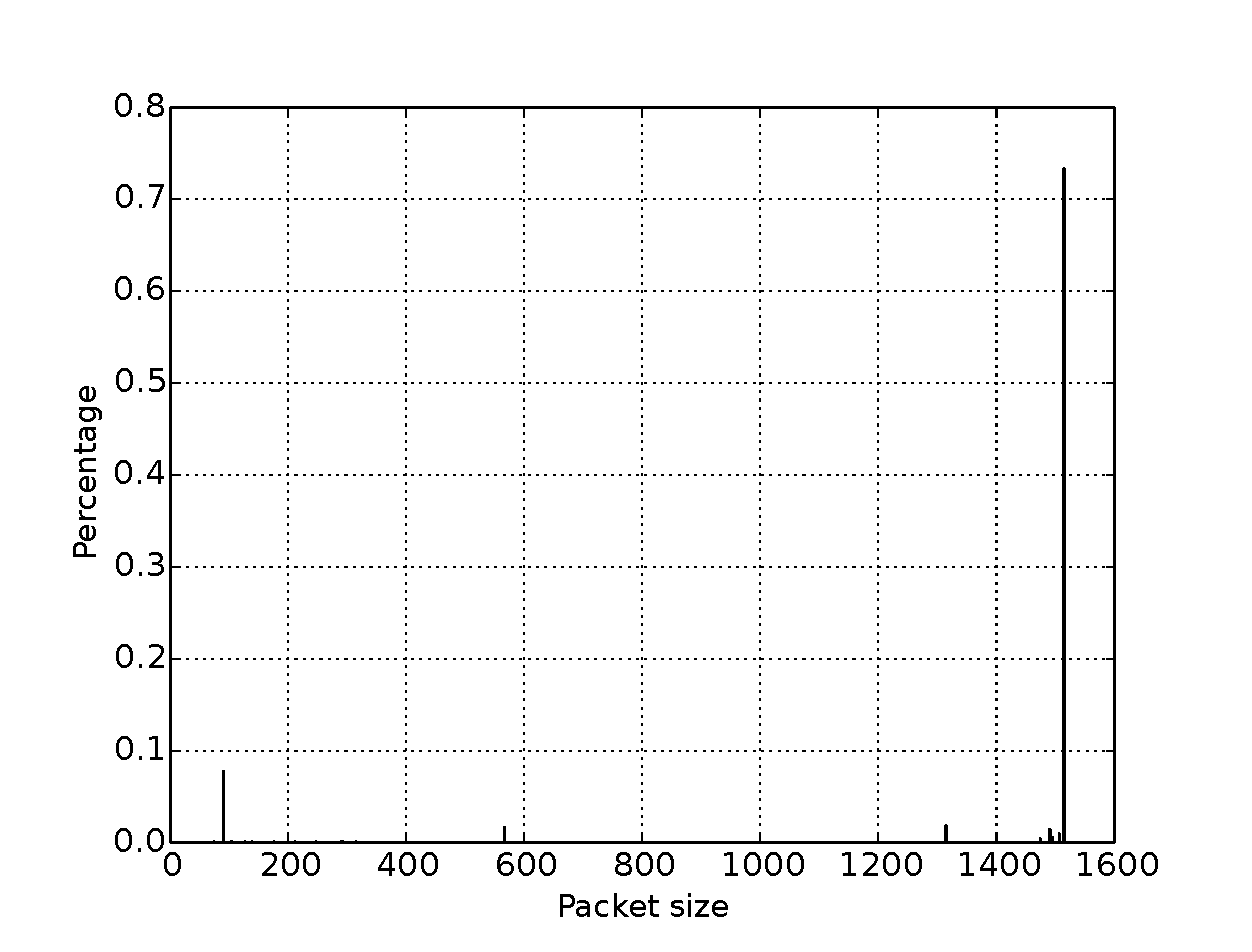
\includegraphics[width=\linewidth]{image/cmpctblock_pktsizes.eps}
\caption{\code{cmpctblock}}
\label{fig:cmpctblock_pktsizes}
\end{subfigure}
\begin{subfigure}{0.24\linewidth}
\centering
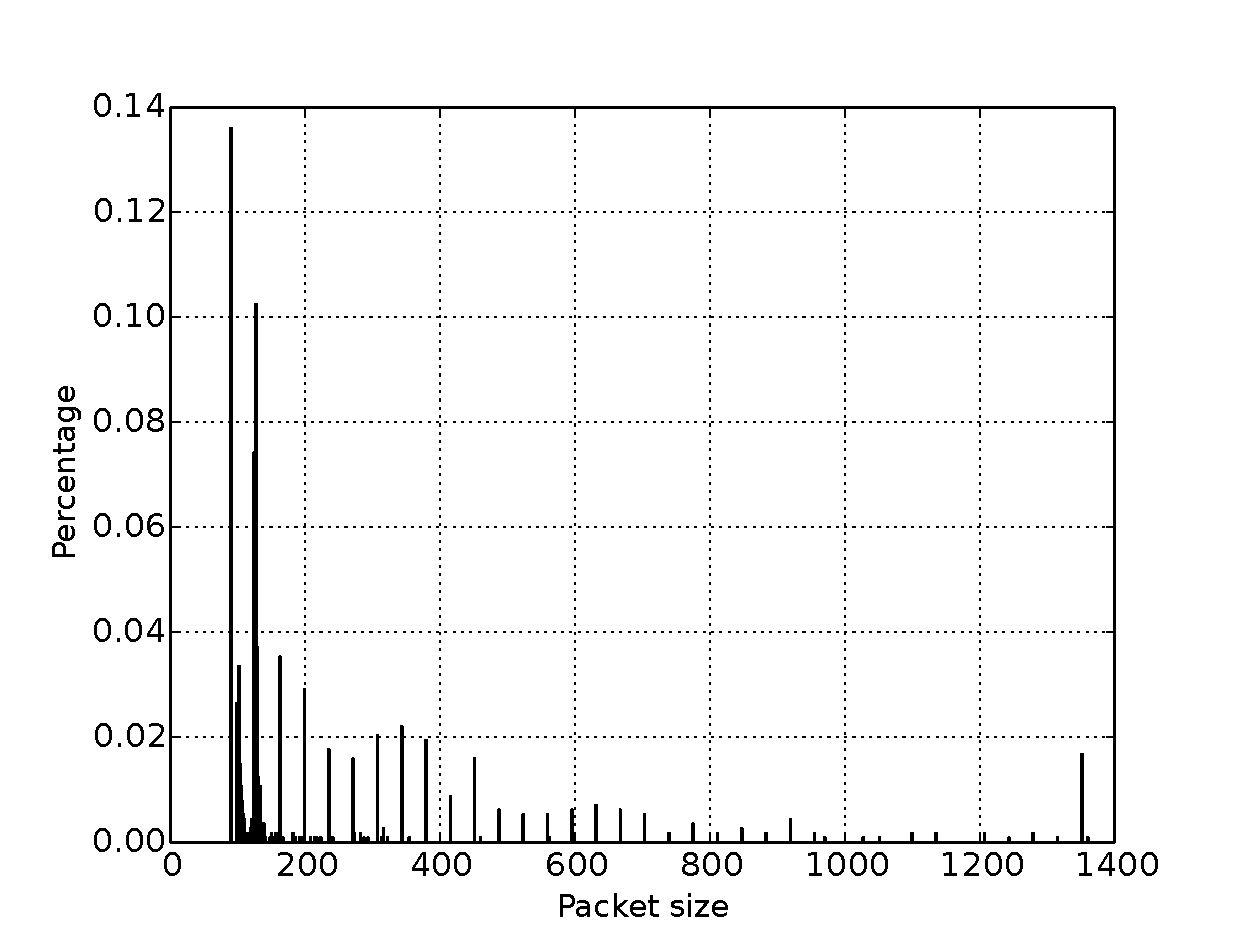
\includegraphics[width=\linewidth]{image/getblocktxn_pktsizes.eps}
\caption{\code{getblocktxn}}
\label{fig:getblocktxn_pktsizes}
\end{subfigure}
\begin{subfigure}{0.24\linewidth}
\centering
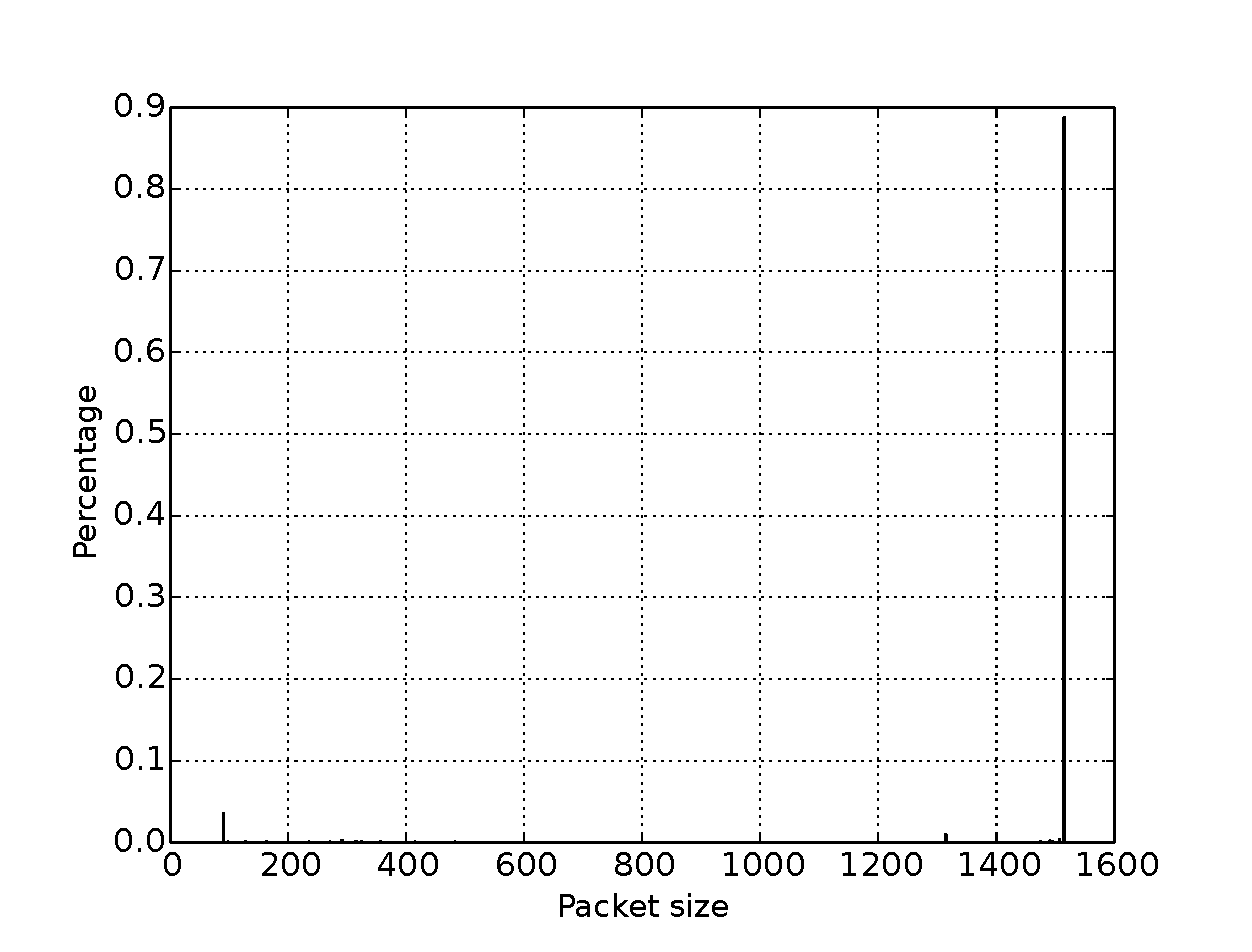
\includegraphics[width=\linewidth]{image/blocktxn_pktsizes.eps}
\caption{\code{blocktxn}}
\label{fig:blocktxn_pktsizes}
\end{subfigure}
\begin{subfigure}{0.24\linewidth}
\centering
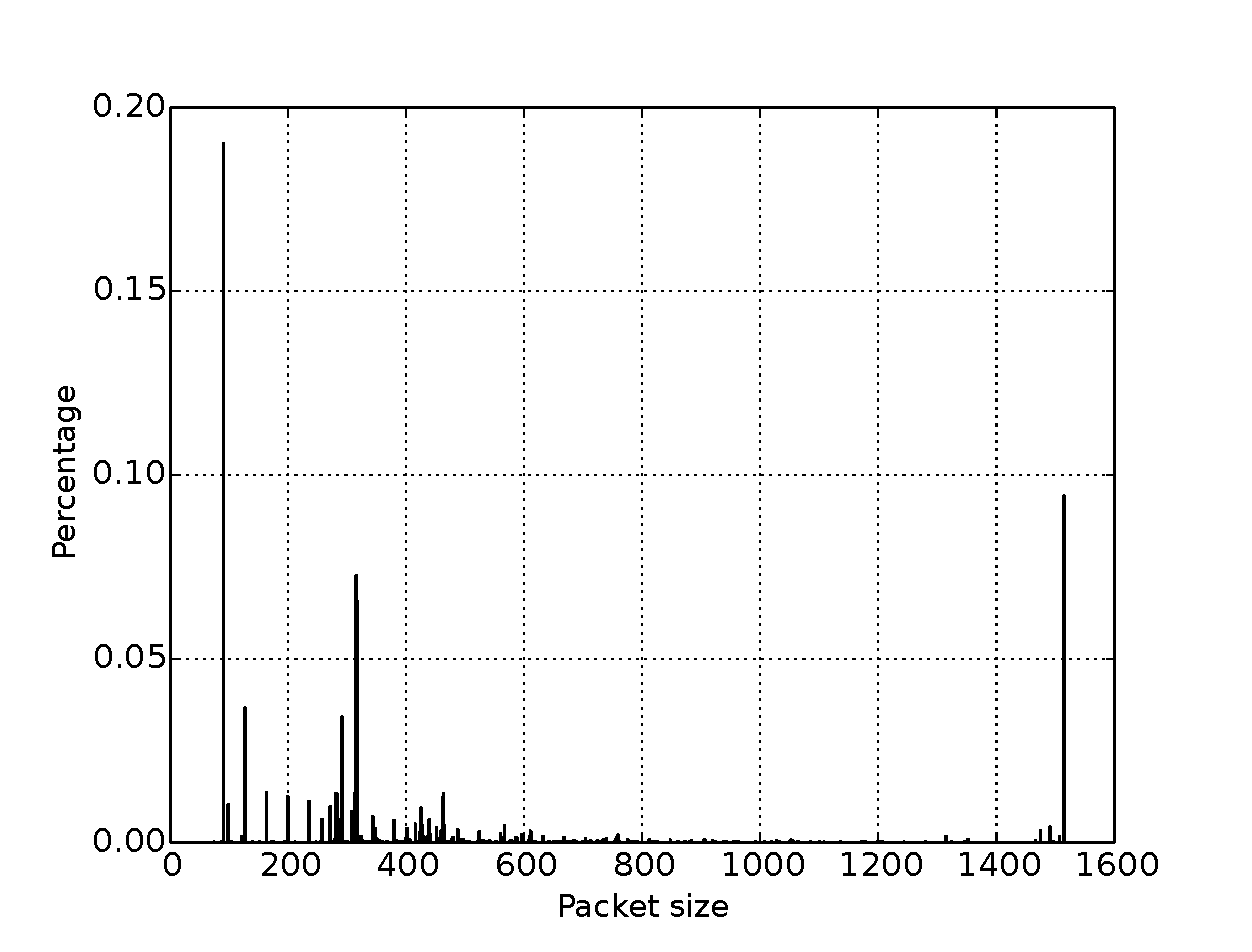
\includegraphics[width=\linewidth]{image/tx_pktsizes.eps}
\caption{\code{tx}}
\label{fig:tx_pktsizes}
\end{subfigure}
\caption{Packet size distribution of \bc communication messages in compact block relaying}\label{fig:sizedist}
\end{figure*}


\begin{figure*}
\centering
\begin{subfigure}{.24\linewidth}
\centering
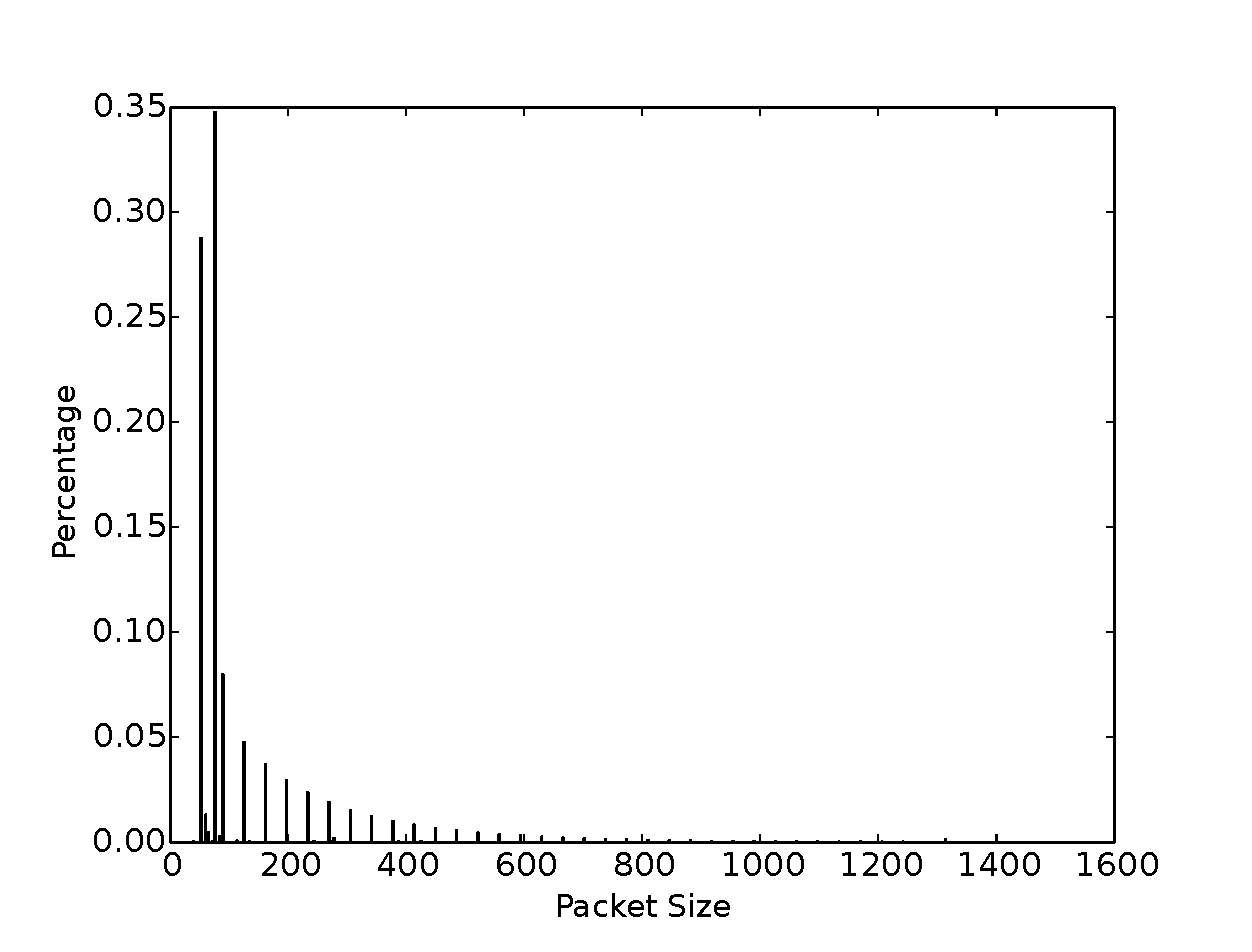
\includegraphics[width=\linewidth]{image/cmpctblock_pkt_size_upstream.eps}
\caption{Compact block, upstream}
\label{fig:aggregate_pkt_size_upstream_cmpct}
\end{subfigure}
\begin{subfigure}{.24\linewidth}
\centering
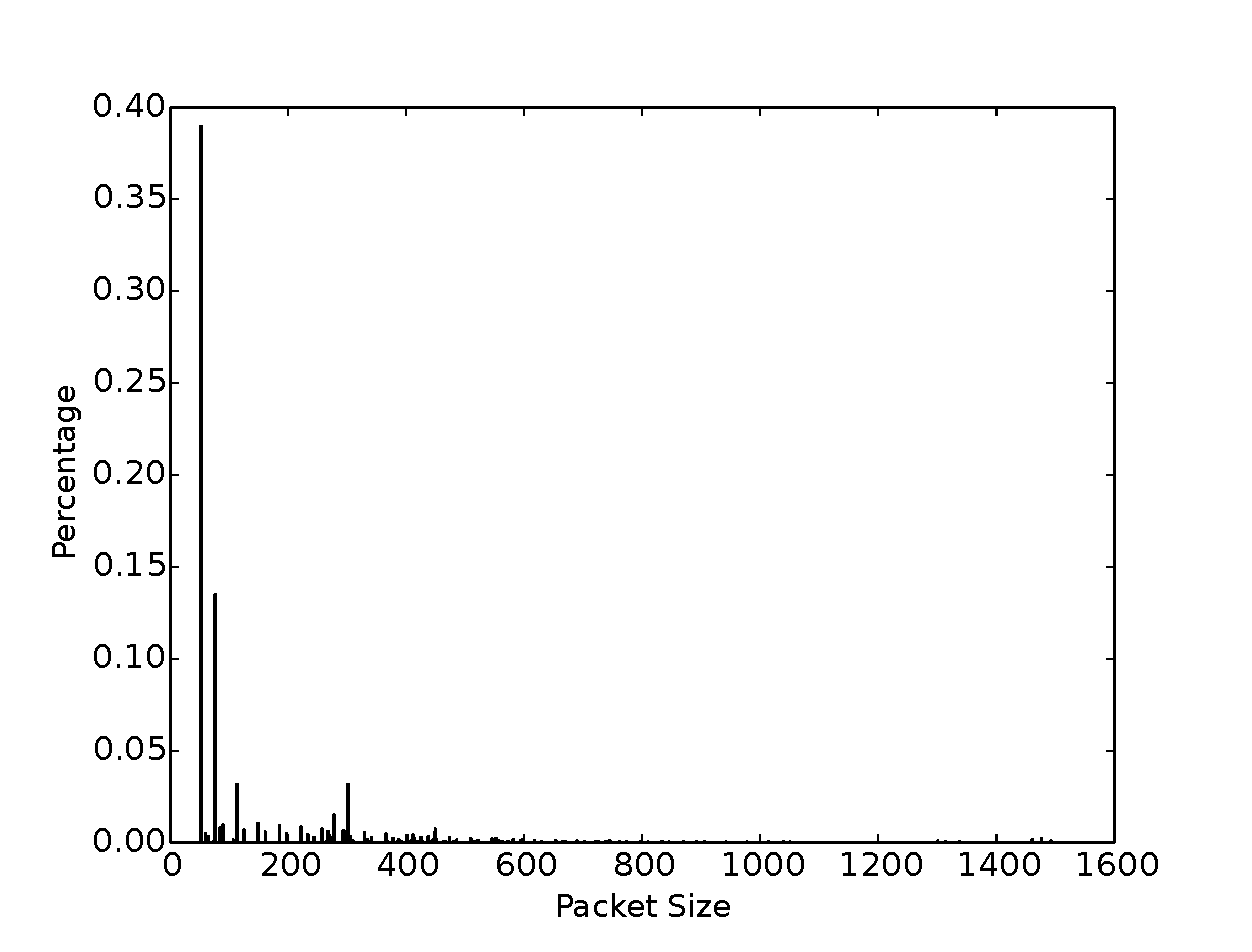
\includegraphics[width=\linewidth]{image/cmpctblock_pkt_size_downstream.eps}
\caption{Compact block, downstream}
\label{fig:aggregate_pkt_size_downstream_cmpct}
\end{subfigure}
\begin{subfigure}{.24\linewidth}
\centering
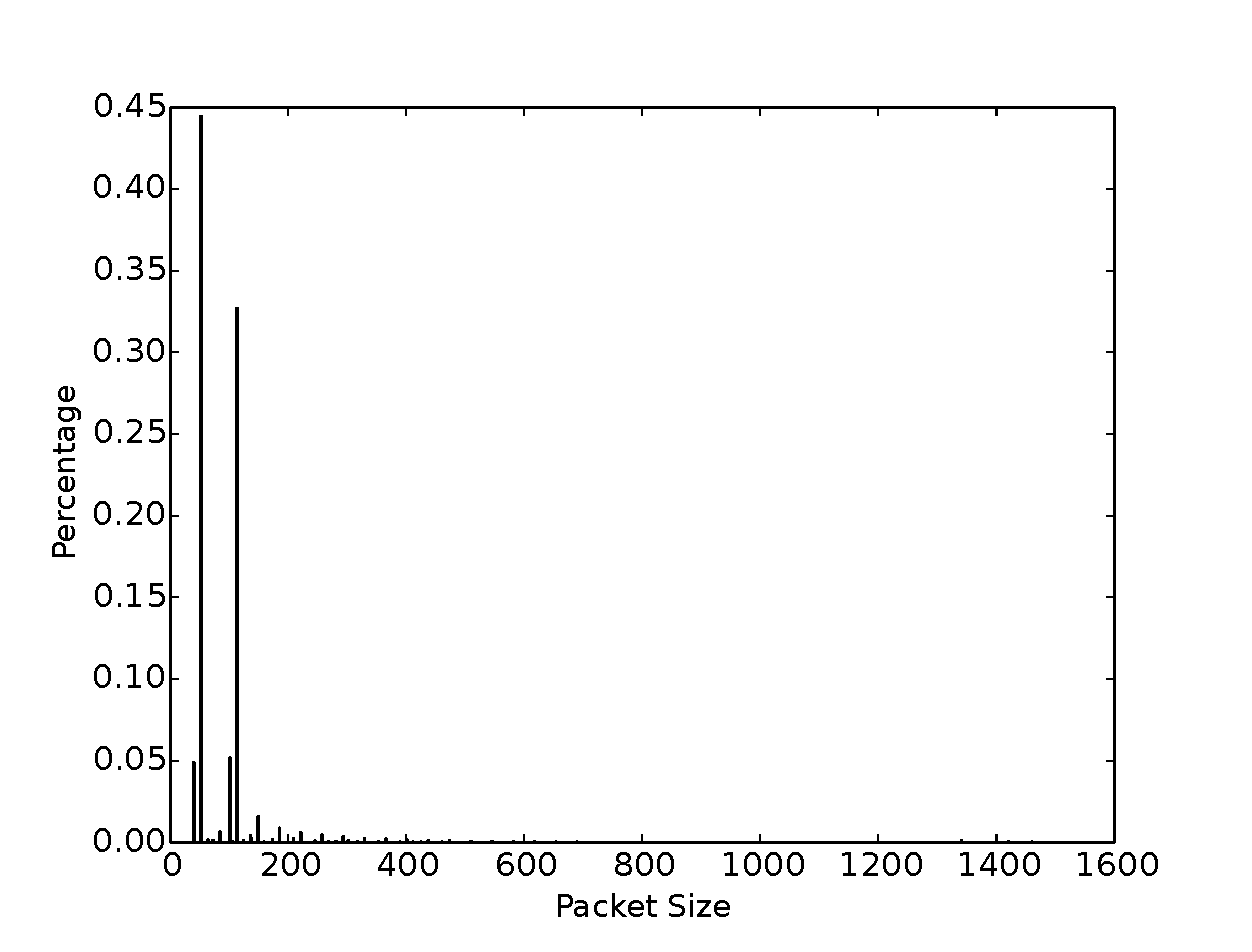
\includegraphics[width=\linewidth]{image/fullblock_pkt_size_upstream.eps}
\caption{Full Block, upstream}
\label{fig:aggregate_pkt_size_upstream_full}
\end{subfigure}
\begin{subfigure}{.24\linewidth}
\centering
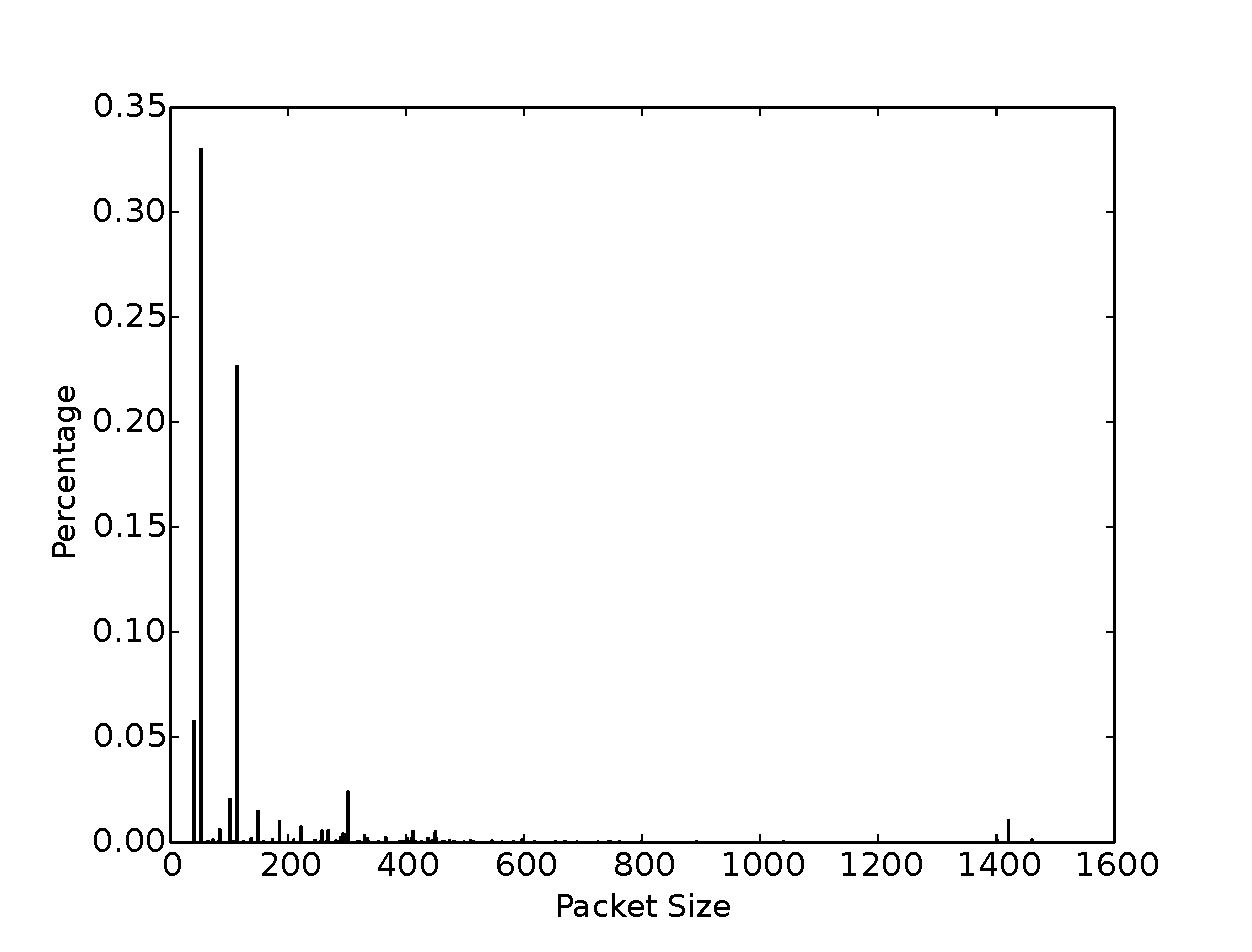
\includegraphics[width=\linewidth]{image/fullblock_pkt_size_downstream.eps}
\captionof{figure}{Full block, downstream}
\label{fig:aggregate_pkt_size_downstream_full}
\end{subfigure}
\begin{subfigure}{.24\linewidth}
\centering
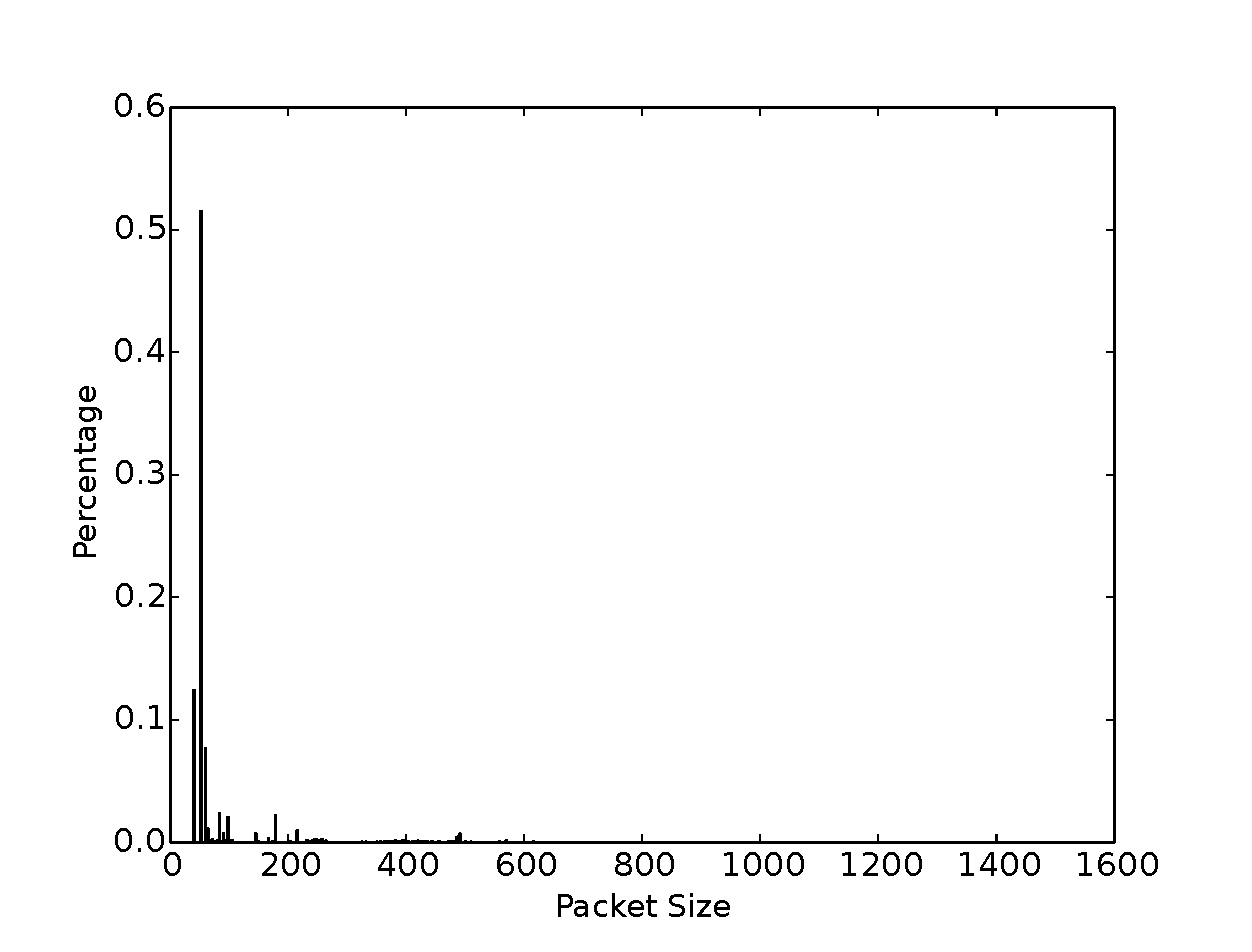
\includegraphics[width=\linewidth]{image/http_pkt_size_upstream.eps}
\caption{HTTP, upstream}
\label{fig:http_pkt_size_upstream}
\end{subfigure}
\begin{subfigure}{.24\linewidth}
\centering
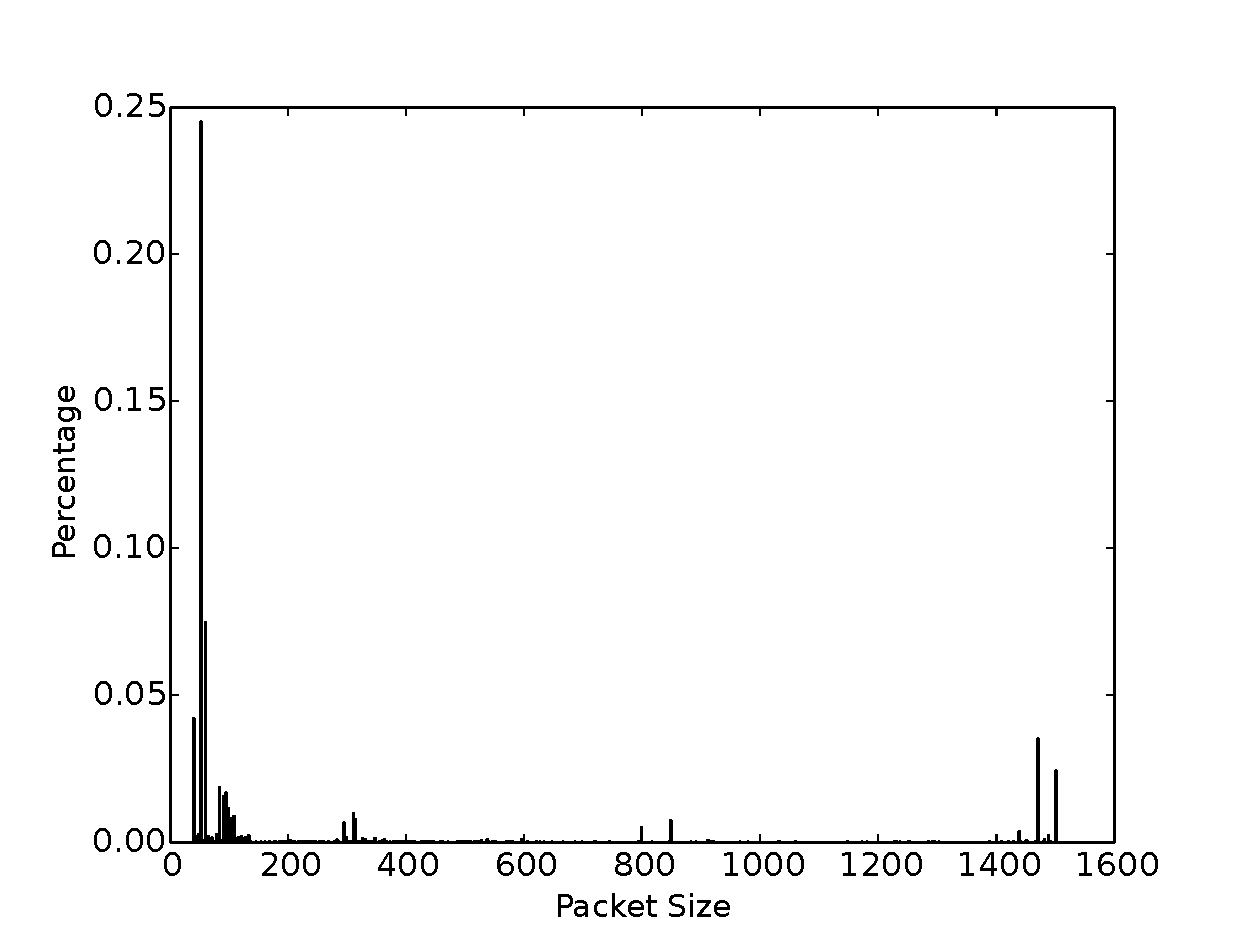
\includegraphics[width=\linewidth]{image/http_pkt_size_downstream.eps}
\caption{HTTP, downstream}
\label{fig:http_pkt_size_downstream}
\end{subfigure}
\begin{subfigure}{.24\linewidth}
\centering
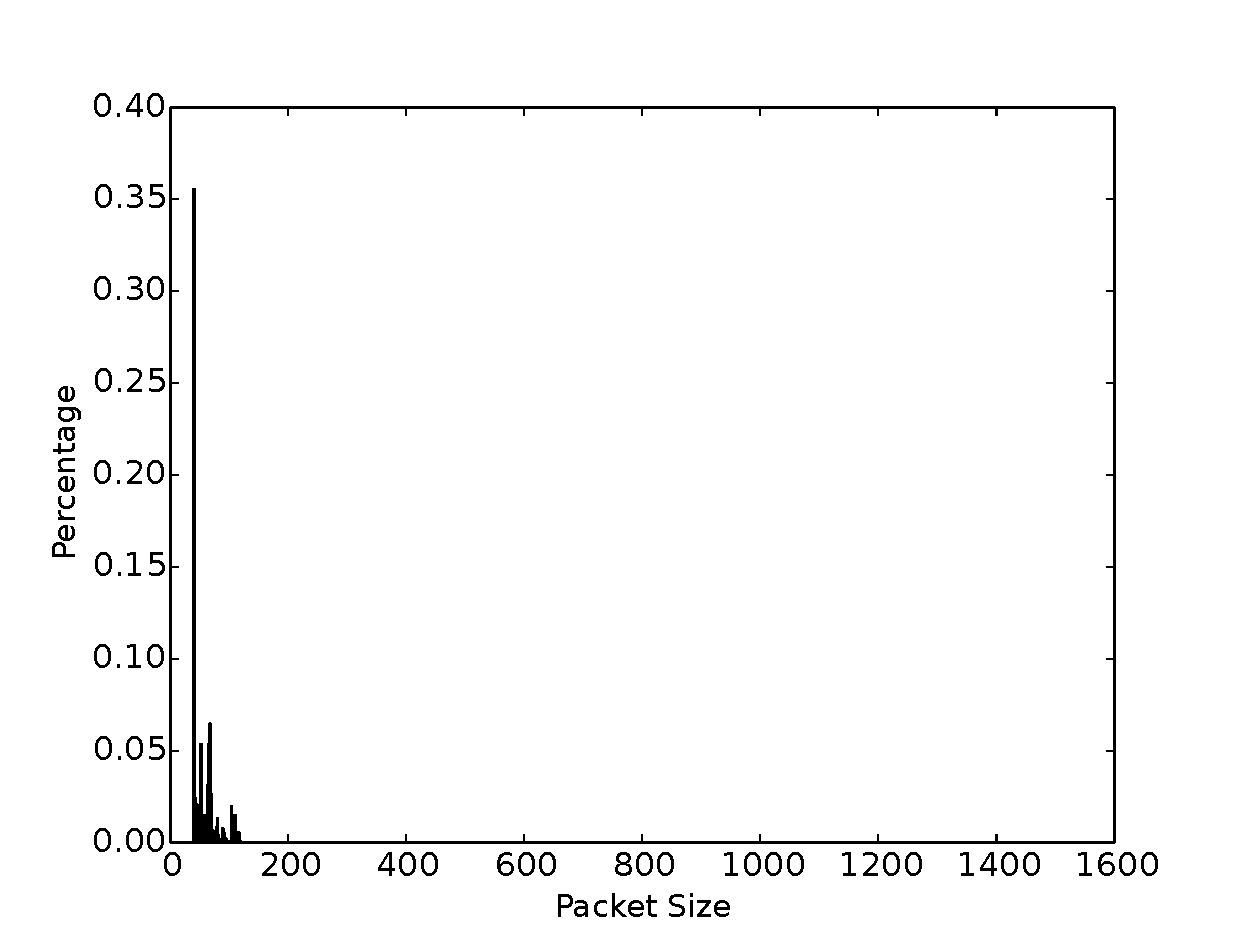
\includegraphics[width=\linewidth]{image/ftp_pkt_size_upstream.eps}
\caption{FTP, upstream}
\label{fig:ftp_pkt_size_upstream}
\end{subfigure}
\begin{subfigure}{.24\linewidth}
\centering
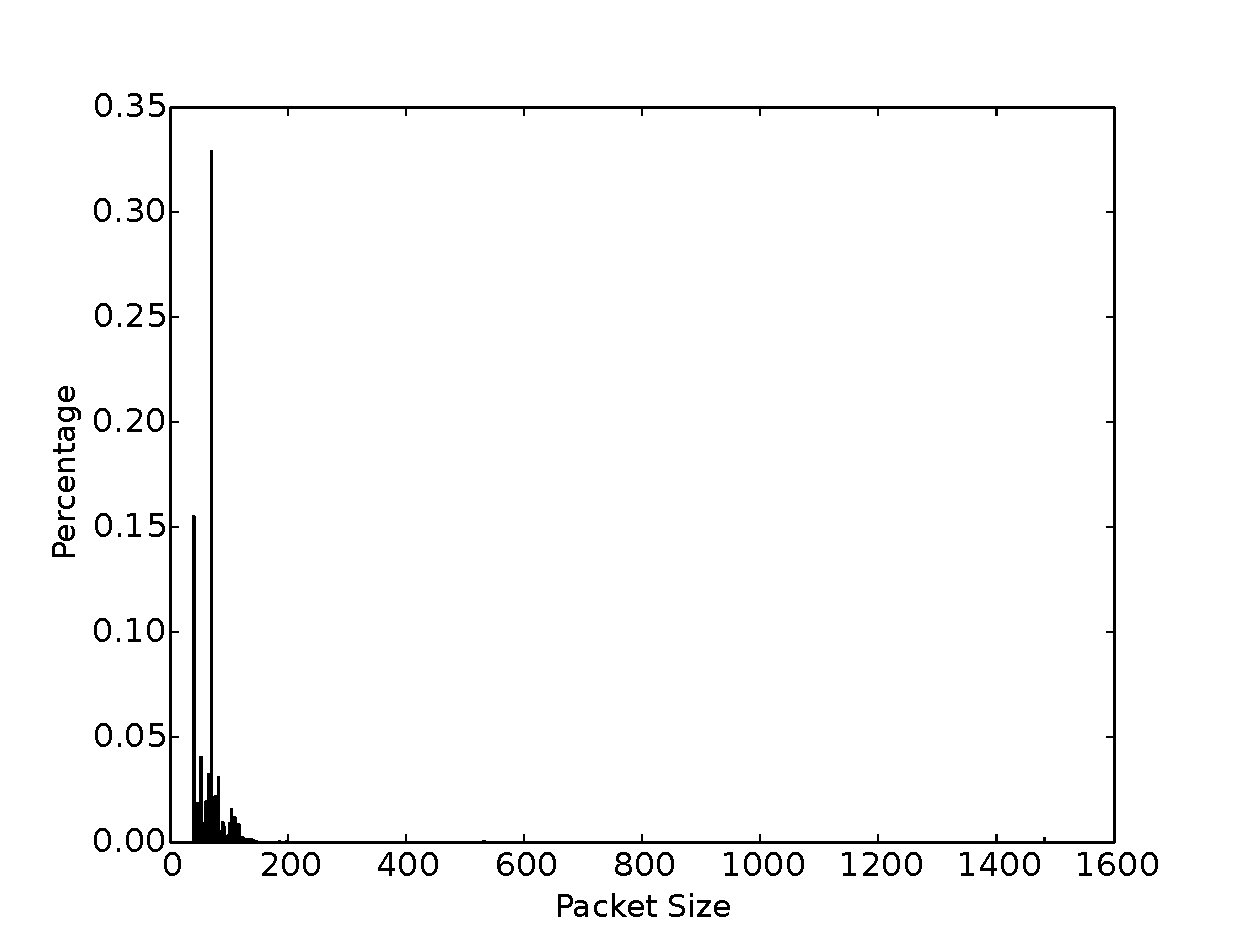
\includegraphics[width=\linewidth]{image/ftp_pkt_size_downstream.eps}
\caption{FTP, downstream}
\label{fig:ftp_pkt_size_downstream}
\end{subfigure}
\begin{subfigure}{.24\linewidth}
\centering
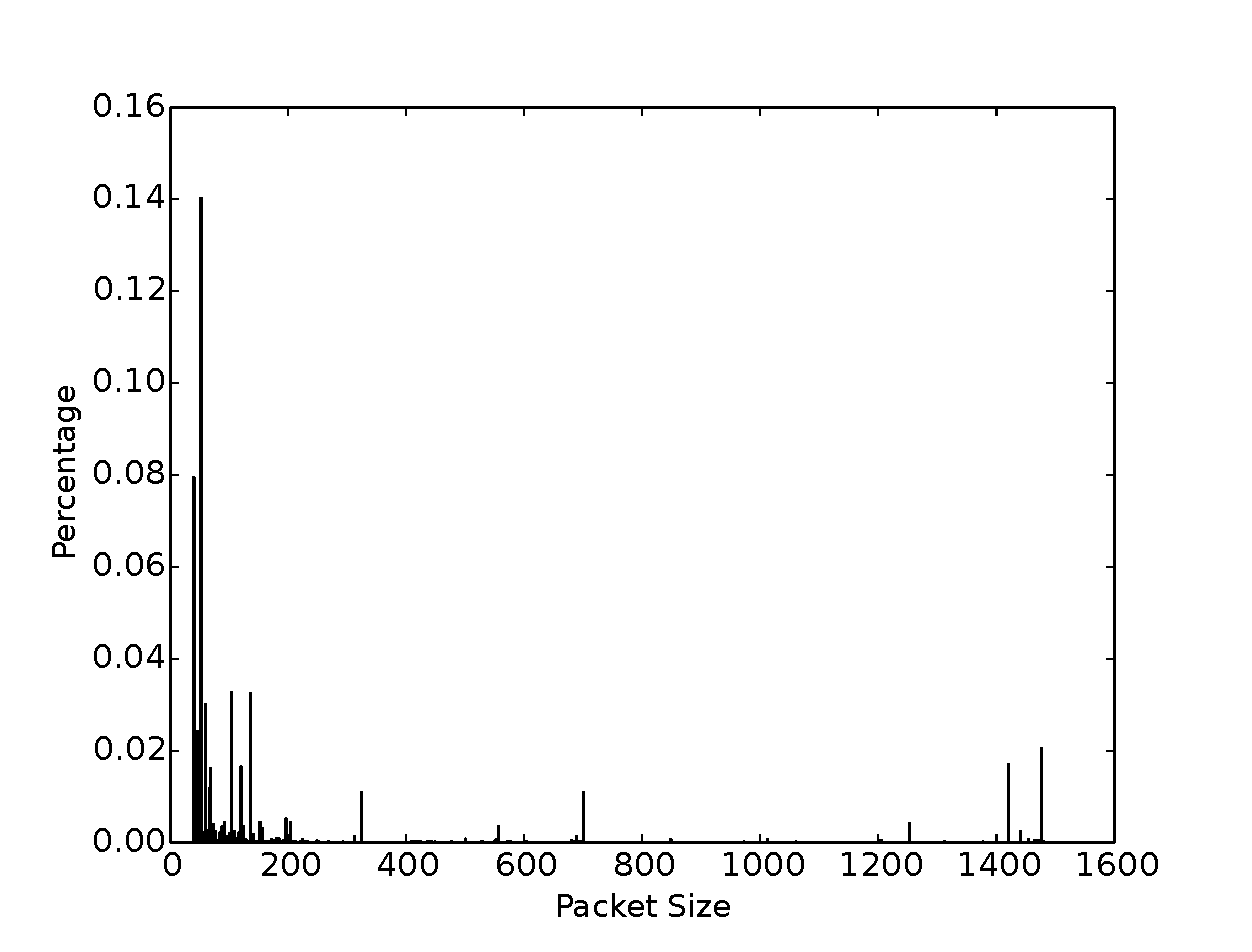
\includegraphics[width=\linewidth]{image/ssh_pkt_size_upstream.eps}
\caption{SSH, upstream}
\label{fig:ssh_pkt_size_upstream}
\end{subfigure}
\begin{subfigure}{.24\linewidth}
\centering
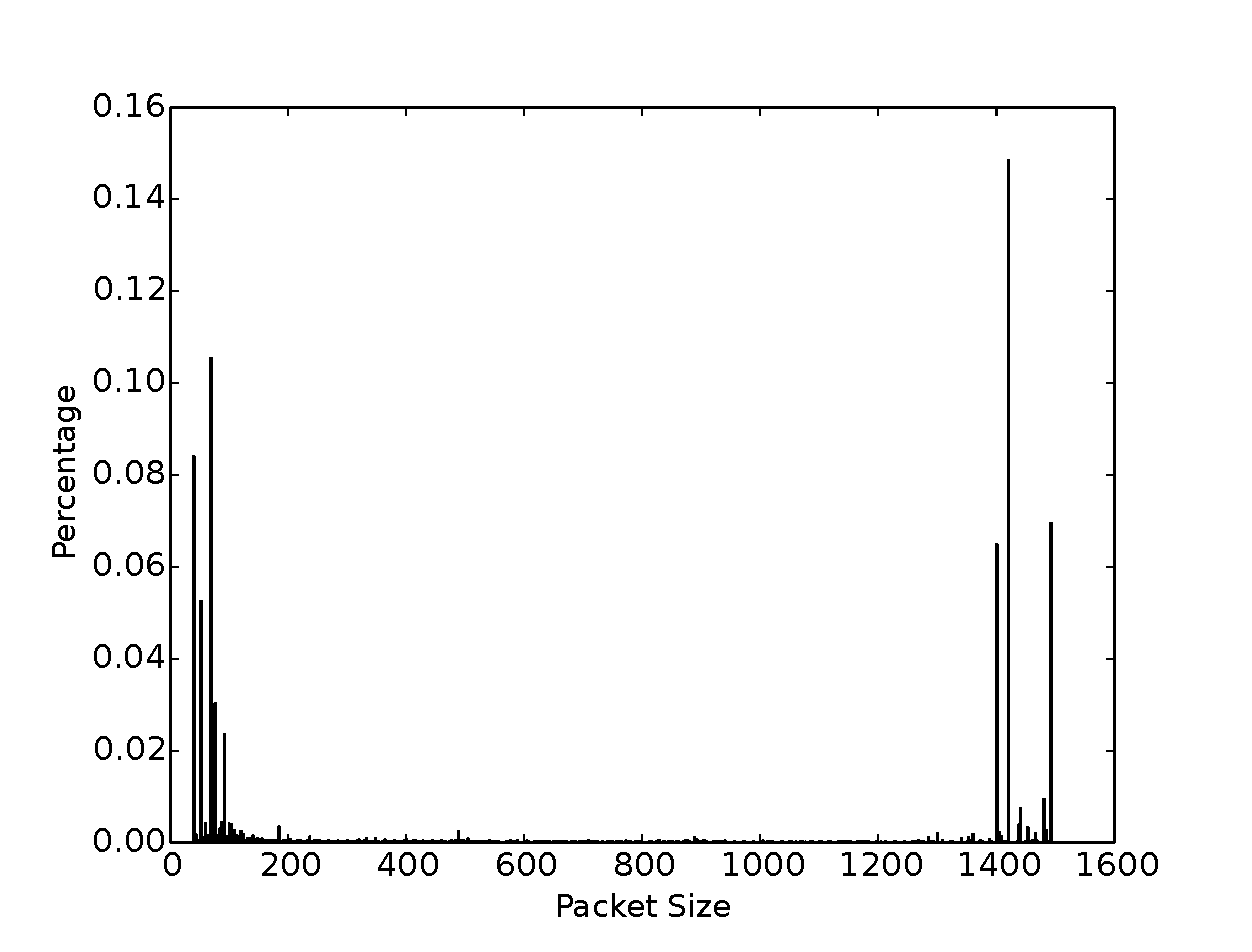
\includegraphics[width=\linewidth]{image/ssh_pkt_size_downstream.eps}
\caption{SSH, downstream}
\label{fig:ssh_pkt_size_downstream}
\end{subfigure}
\begin{subfigure}{.24\linewidth}
\centering
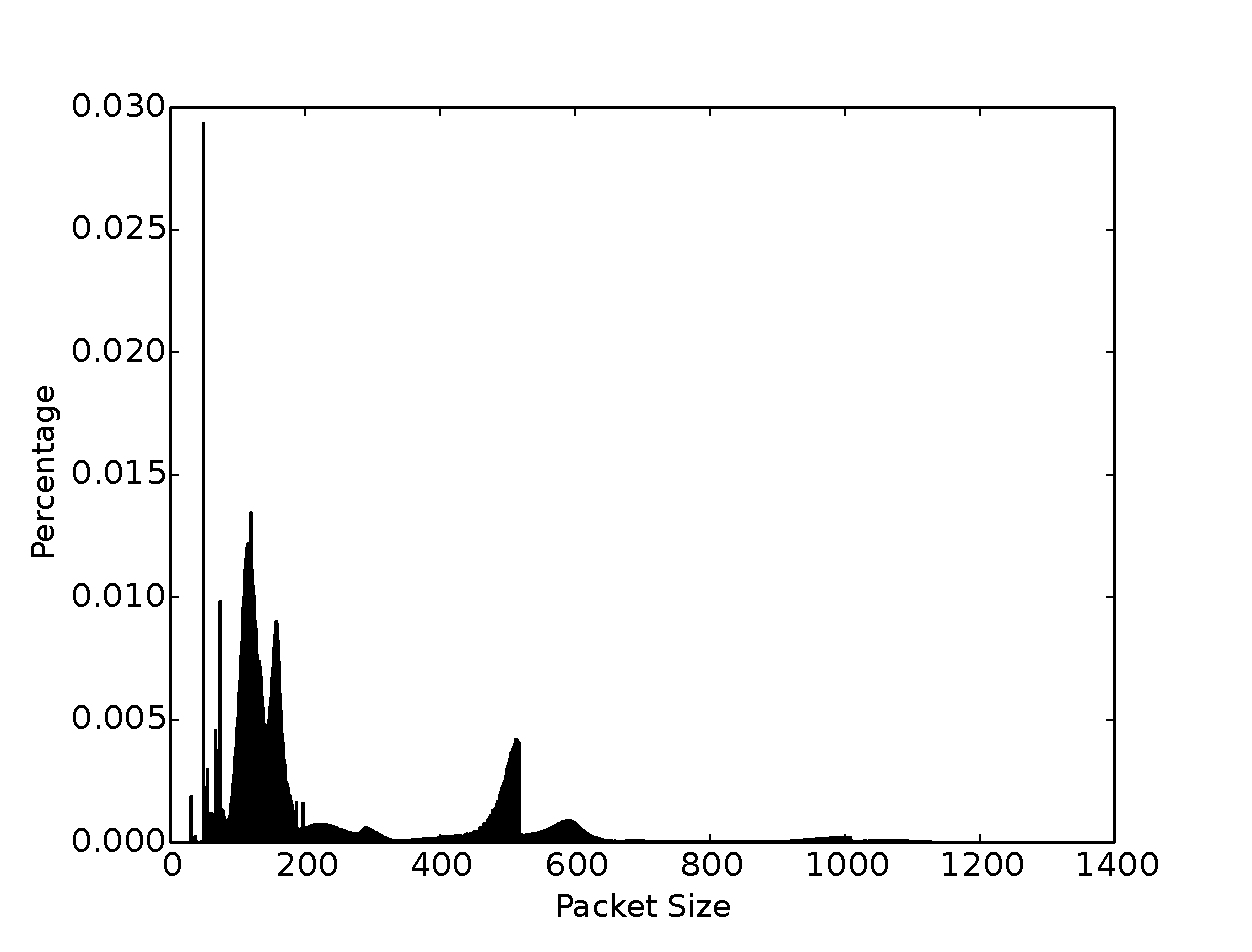
\includegraphics[width=\linewidth]{image/voip_pkt_size_upstream.eps}
\caption{VoIP, upstream}
\label{fig:voip_pkt_size_upstream}
\end{subfigure}
\begin{subfigure}{.24\linewidth}
\centering
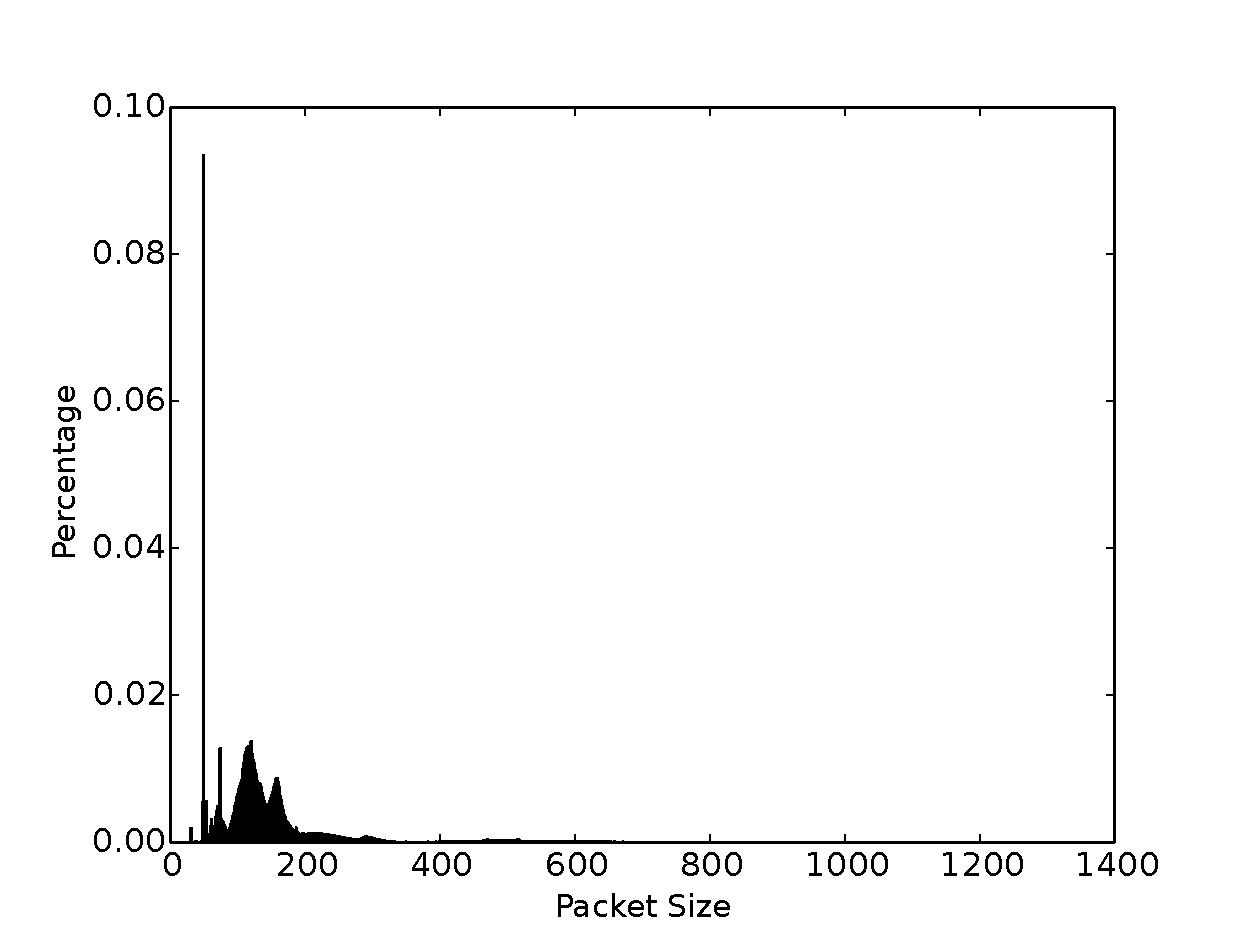
\includegraphics[width=\linewidth]{image/voip_pkt_size_downstream.eps}
\captionof{figure}{VoIP, downstream}
\label{fig:voip_pkt_size_downstream}
\end{subfigure}
\begin{subfigure}{.24\linewidth}
\centering
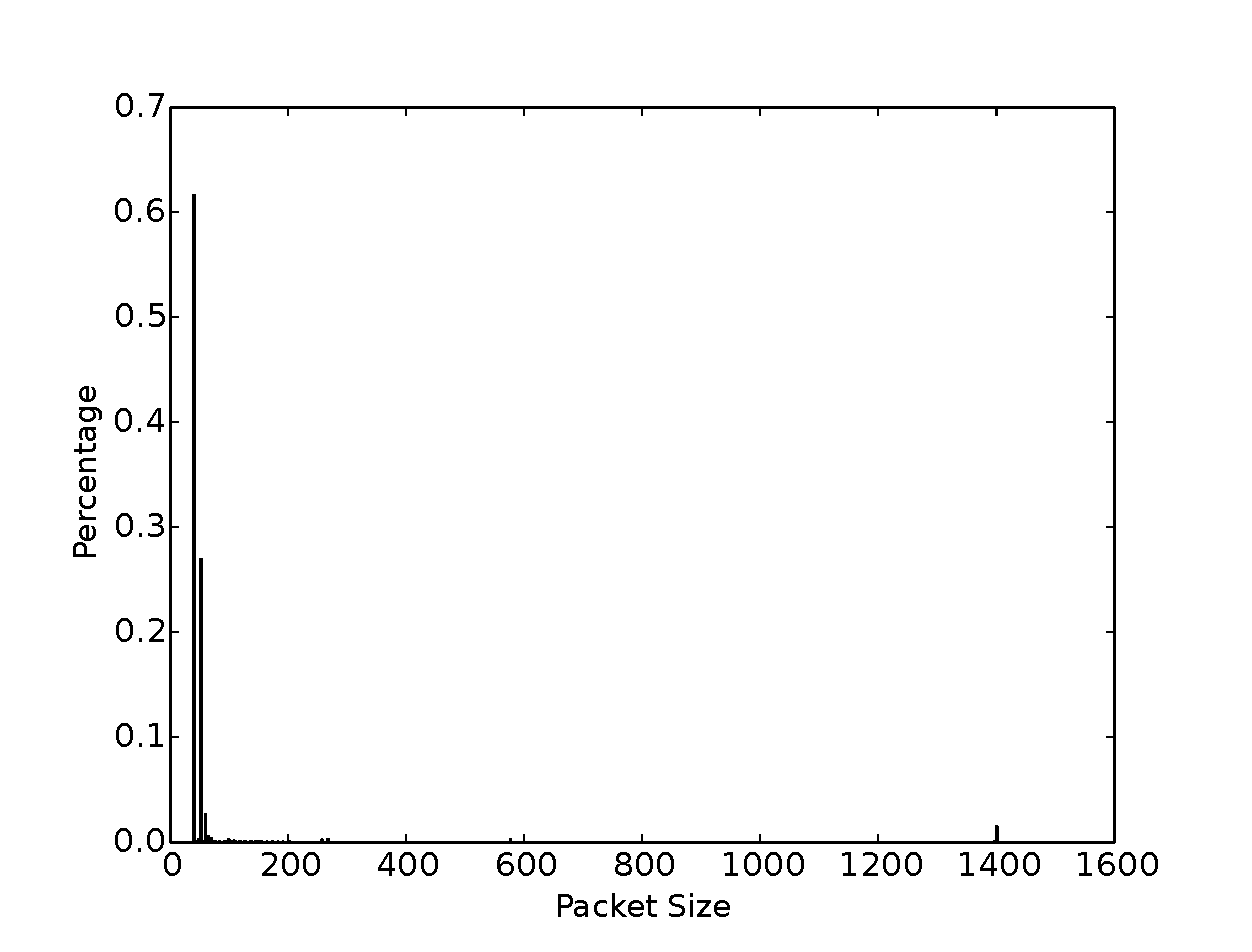
\includegraphics[width=\linewidth]{image/bittorrent_pkt_size_upstream.eps}
\caption{BitTorrent, upstream}
\label{fig:bittorrent_pkt_size_upstream}
\end{subfigure}
\begin{subfigure}{.24\linewidth}
\centering
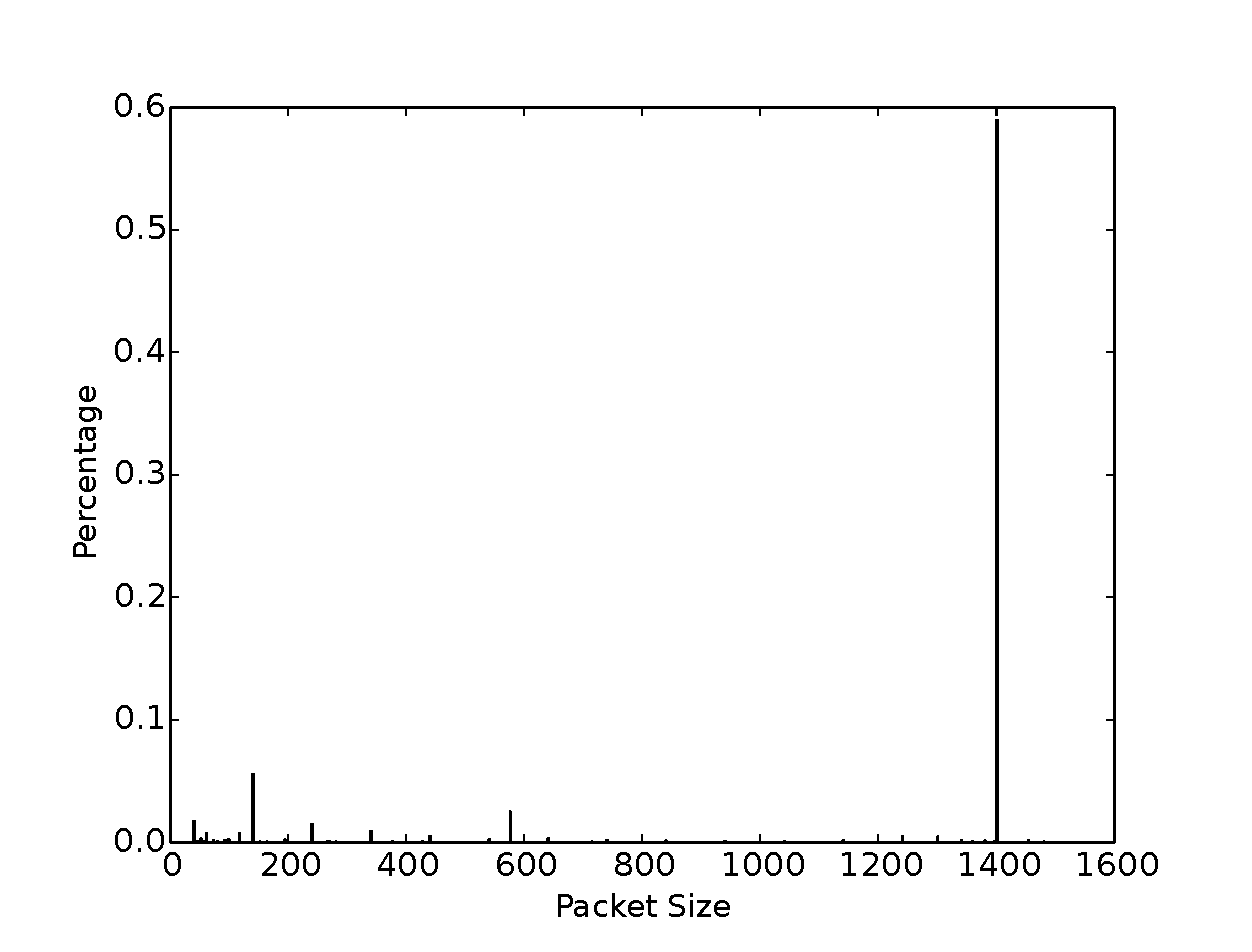
\includegraphics[width=\linewidth]{image/bittorrent_pkt_size_downstream.eps}
\caption{BitTorrent, downstream}
\label{fig:bittorrent_pkt_size_downstream}
\end{subfigure}
\caption{Upstream and downstream packet size distribution of \bc and several popular protocols}\label{fig:traff-hist}
\end{figure*}

%\subsection{Ratio of Downstream to Upstream}\label{apend:ratio}


\subsection{Proportion and Distribution of Messages} \label{sec:prop_dist_msg}

As discussed in the previous section, \bc peers generate various kinds of messages. 
We show that the distribution and sizes of such messages are quite unique to the \bc protocol, 
distinguishing \bc traffic reliably from other protocols. 


Table~\ref{table:msg_proportion} demonstrates the proportion of different messages in the \bc traffic we collected 
for 31 days. As can be seen, \code{tx} and \code{inv} are dominating with 43.6\% and 27.2\% of all packets, respectively. 
Therefore, the characteristics of these messages will shape the pattern of a \bc peer's traffic. 



\paragraphb{Distribution of Packet Sizes.}
Figures~\ref{fig:inv_pktsizes} to~\ref{fig:tx_pktsizes} illustrate
the  packet size histogram of 
different types of \bc messages in our collected \bc traffic.
As can be seen, each type of message has a distinguishing traffic pattern. 


\paragraphb{Histogram of packet sizes in aggregate traffic.}
Figures~\ref{fig:aggregate_pkt_size_upstream_cmpct} and~\ref{fig:aggregate_pkt_size_downstream_cmpct} show the histogram of packet sizes in the upstream and downstream directions, respectively, in compact block relaying. 
As mentioned before, \code{tx} and \code{inv} dominate the messages sent by a typical \bc peer, therefore, their sizes 
(shown in Figures~\ref{fig:inv_pktsizes} and \ref{fig:tx_pktsizes}) strongly shape the histogram of \bc traffic, making them uniquely distinguishable from other protocols. 

We also show the histogram of \bc traffic in the full block relaying mode in Figures~\ref{fig:aggregate_pkt_size_upstream_full} and~\ref{fig:aggregate_pkt_size_downstream_full}. These histograms have a larger spike close to the MTU, unlike the case of compact block relaying. These are because of the larger block sizes (around 1MB) in the full block relaying. 

\paragraphe{Comparing to other protocols:}
Figures~\ref{fig:http_pkt_size_upstream} to~\ref{fig:bittorrent_pkt_size_downstream}  show the histogram of other popular protocols, collected as described in Section~\ref{sec:exp-dataset}. Note that we look at the traffic after going through an encryption tunnel, e.g., a VPN or SSH tunnel, so the histogram includes the (small) TCP ACK packets. 

As we can see, 
the packet size distribution of \bc is uniquely different from these other protocols, since a \bc connection is composed of unique messages with specific size distributions shown before. For instance, the large number of \code{inv} messages shapes the overall distribution of sizes in \bc traffic. 

 

\paragraphb{Ratio of Downstream to Upstream.}
We also measured the ratio of downstream to upstream traffic volume, which is shown in Figure~\ref{fig:ratio_downstream_upstream_traffic_volume_bitcoin}.
Unlike other protocols like HTTP (shown in
Figures~\ref{fig:ratio_downstream_upstream_traffic_volume_http} to \ref{ratio_downstream_upstream_traffic_volume_bittorrent}),
\bc traffic has a \emph{symmetric} traffic volume in upstream and downstream. 
This is due to the fact that \bc peers broadcast most of the bulky protocol messages they receive such as block and transaction announcements. 


\subsection{Shape of Traffic}\label{sec:shape_of_traffic}
\begin{figure*}
\centering
\begin{subfigure}{0.32\linewidth}
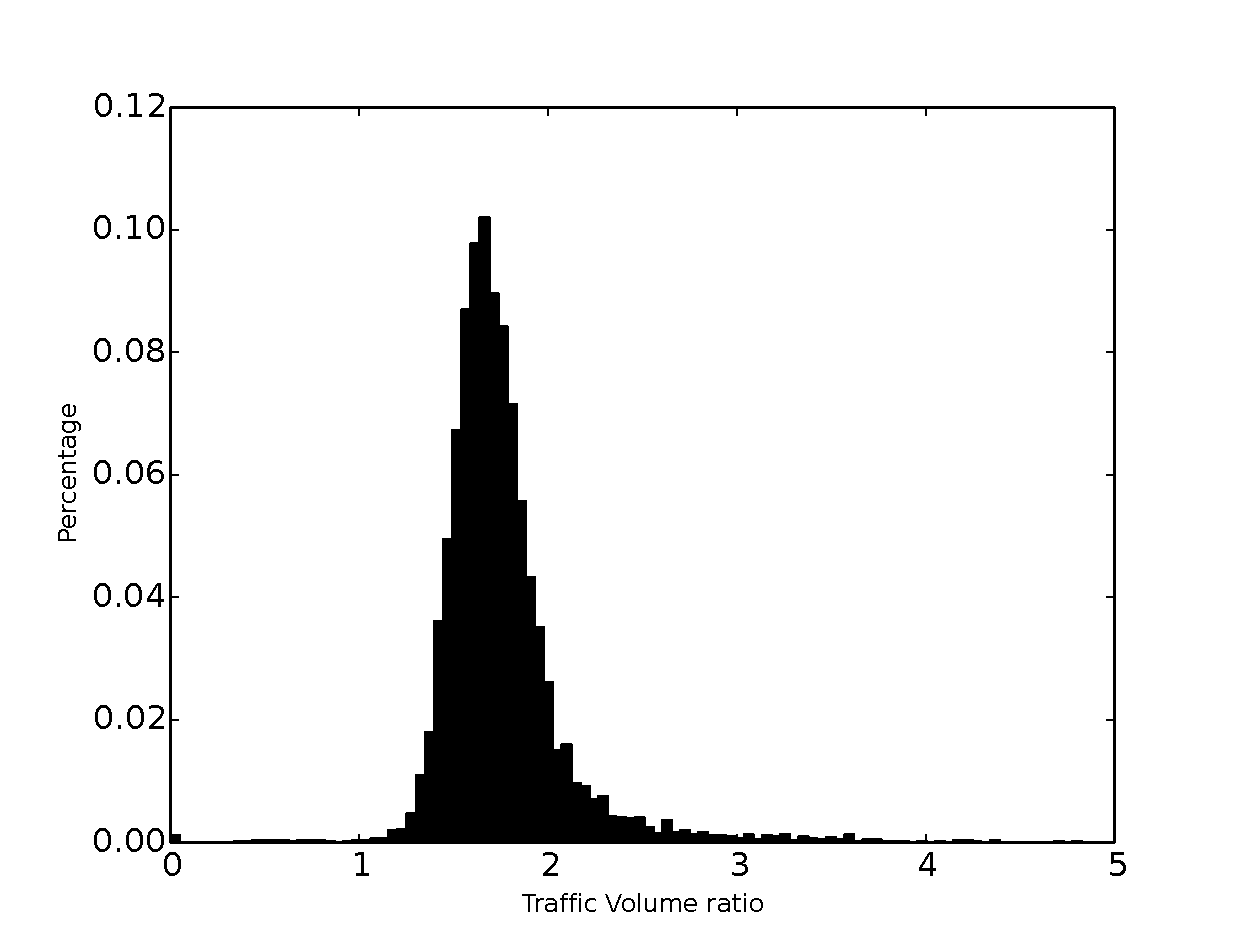
\includegraphics[width=\linewidth]{image/ratio_downstream_upstream_traffic_volume_bitcoin.eps}
\caption{Bitcoin, ratio per 5 minutes traffic}
\label{fig:ratio_downstream_upstream_traffic_volume_bitcoin}
\end{subfigure}
\begin{subfigure}{0.32\linewidth}
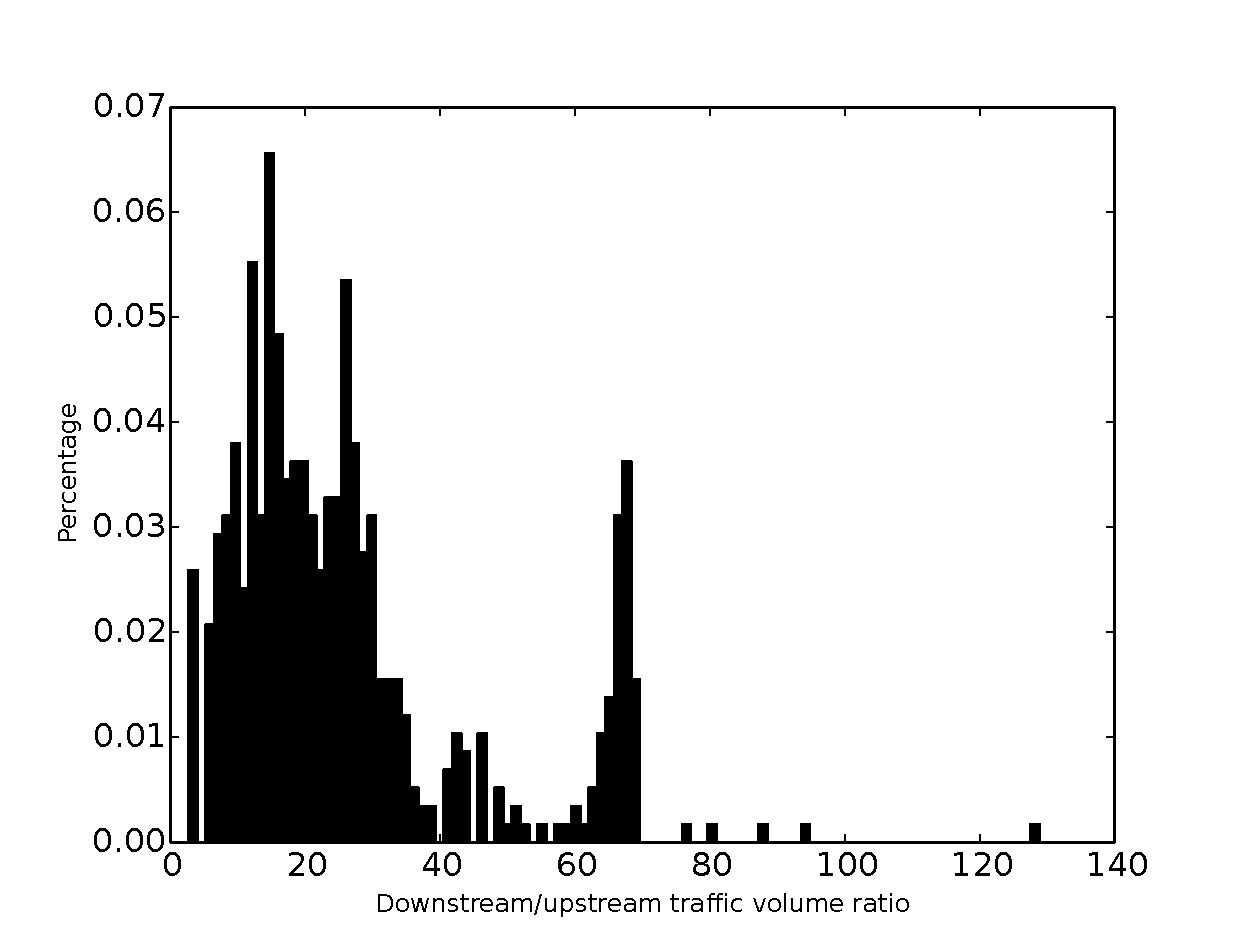
\includegraphics[width=\linewidth]{image/ratio_downstream_upstream_traffic_volume_http.eps}
\caption{HTTP, ratio per website}
\label{fig:ratio_downstream_upstream_traffic_volume_http}
\end{subfigure}
\begin{subfigure}{0.32\linewidth}
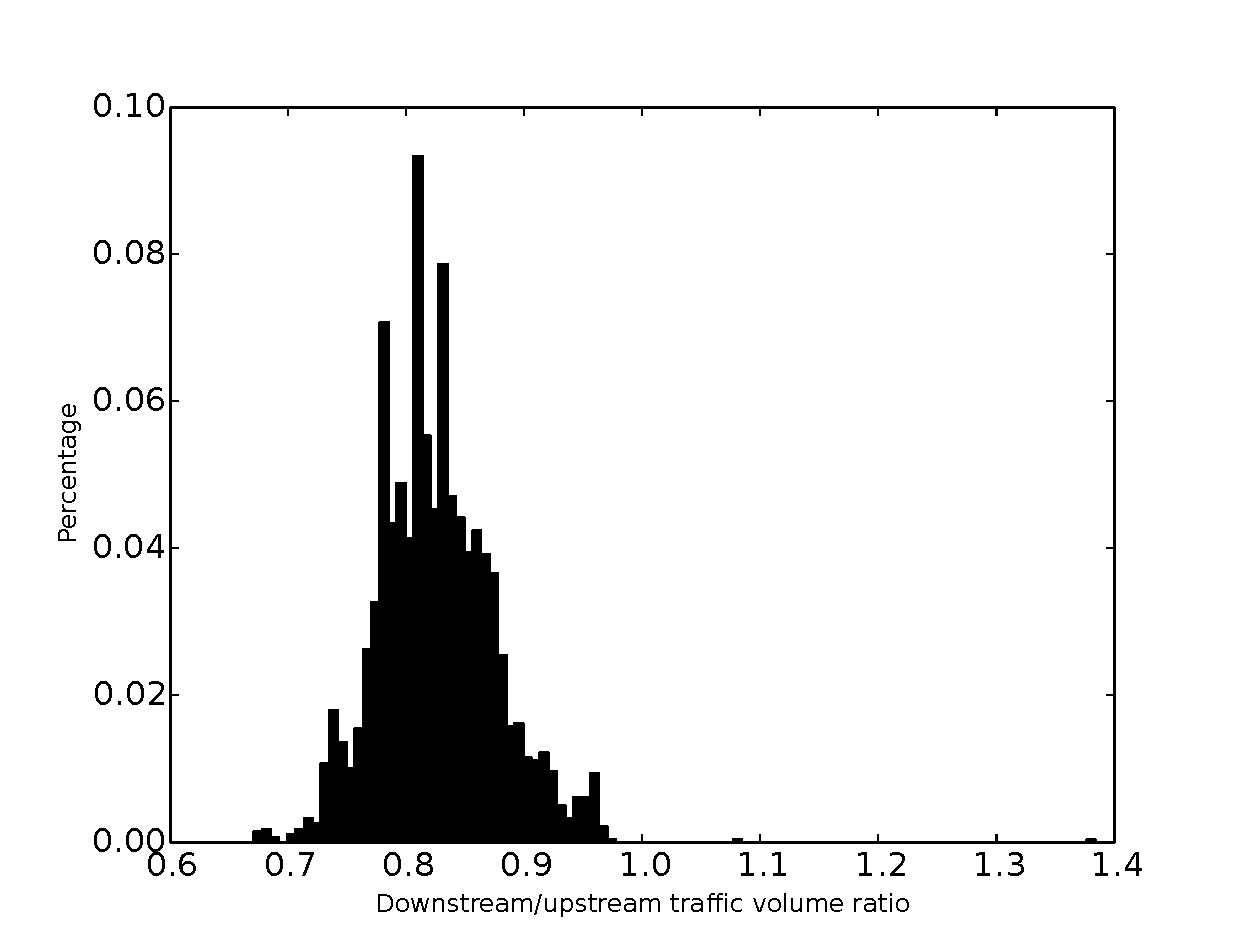
\includegraphics[width=\linewidth]{image/ratio_downstream_upstream_traffic_volume_ftp.eps}
\caption{FTP, ratio per 5 minutes traffic}
\label{ratio_downstream_upstream_traffic_volume_ftp}
\end{subfigure}
\begin{subfigure}{0.32\linewidth}
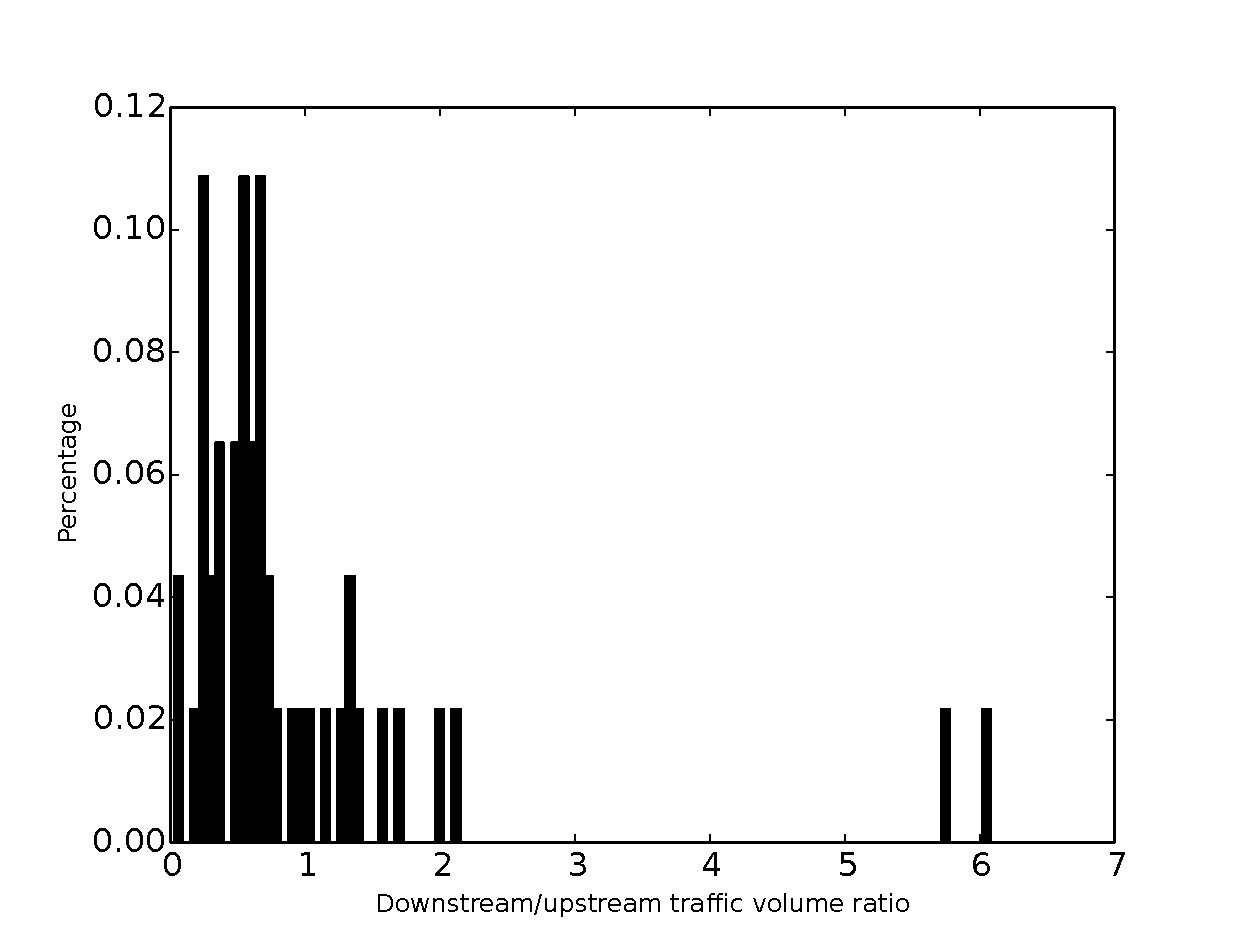
\includegraphics[width=\linewidth]{image/ratio_downstream_upstream_traffic_volume_ssh.eps}
\caption{SSH, ratio per 1 minute traffic}
\label{ratio_downstream_upstream_traffic_volume_ssh}
\end{subfigure}
\begin{subfigure}{0.32\linewidth}
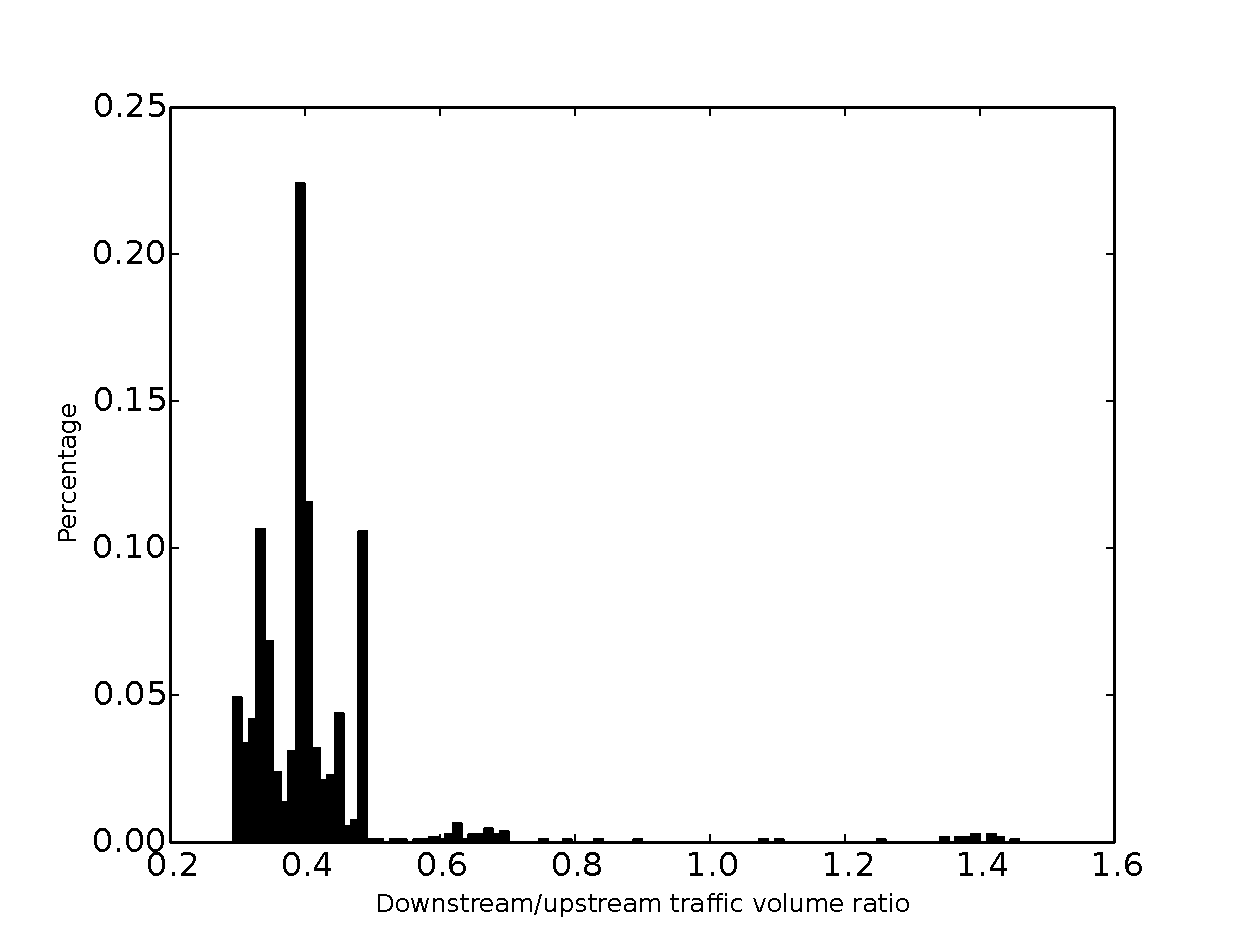
\includegraphics[width=\linewidth]{image/ratio_downstream_upstream_traffic_volume_voip.eps}
\caption{VoIP, ratio per 5 minutes traffic}
\label{ratio_downstream_upstream_traffic_volume_voip}
\end{subfigure}
\begin{subfigure}{0.32\linewidth}
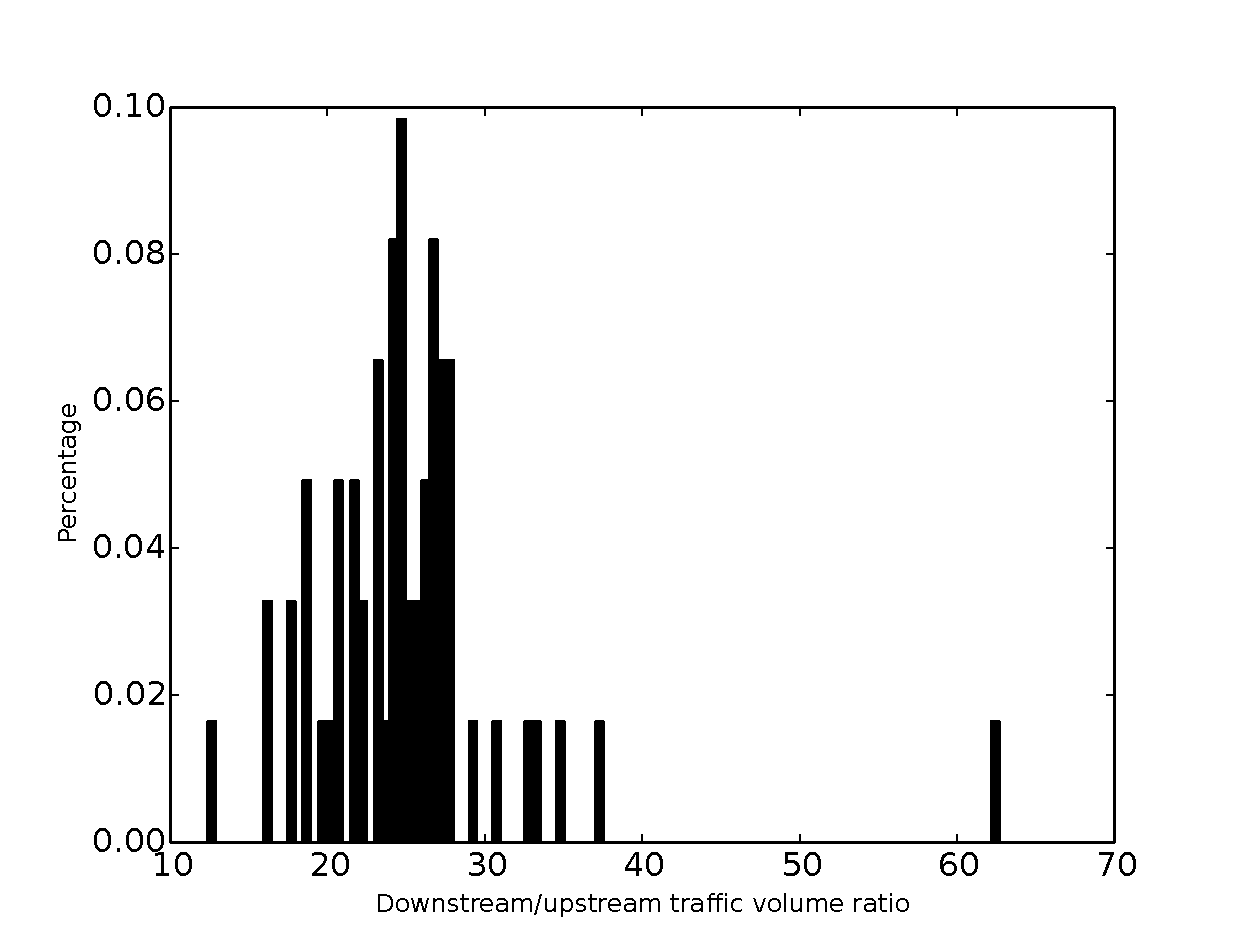
\includegraphics[width=\linewidth]{image/ratio_downstream_upstream_traffic_volume_bittorrent.eps}
\caption{BitTorrent, ratio per 5 minutes traffic}
\label{ratio_downstream_upstream_traffic_volume_bittorrent}
\end{subfigure}
\caption{Ratio of downstream to upstream traffic volume}
\end{figure*}
Above we showed that the counts and sizes of packets in \bc demonstrate a unique behavior. 
In addition, the shape of traffic in \bc and the volume of traffic received over time  is distinguishable from other protocols.

\paragraphb{Full block relaying mode} 
Figure~\ref{fig:bitcoin_traffic_pattern} shows the traffic of a \bc client operating in the full block relaying mode.
As can be seen, the small protocol packets, mostly corresponding to \code{inv} and \code{tx} messages, appear 
uniformly over the time. 
On the other hand, the \bc full blocks appear as large spikes of roughly 1MB at specific points in time, i.e., once a new block is generated in the network. 

\paragraphb{Compact block relaying mode}
In the compact block relaying mode, it would be harder to notice the block spikes, 
since only a sketch of the blocks is transmitted. In this mode, transmitting a compact block in the network results in smaller spikes of 100KB. Spikes of such small sizes may also occur when unverified transactions are transmitted, which will increase the detection's false positive. Also, a \bc client may operate in the high bandwidth mode, in which the receiver node  asks its peers to send new blocks without asking for permissions first. This will lead to more than one peer sending the same block at the same time. This and the large volume of missed transactions result in having spikes with more than 100 KB in the traffic. 
Figure~\ref{fig:cmpctblock_traffic_volume_detectable} illustrates  when and how
compact blocks appear on a peer's traffic. As can be seen, compact blocks appear at
smaller amplitudes than the actual block size, but the behavior is also nondeterministic,
since it depends on whether the client has previously received some of the transactions
in that block. This intuitively makes detection of compact blocks less reliable than full blocks, as shown later in our experiments. 

We also measure the size of compact blocks by measuring the 
\textit{length} field of \code{cmpctblock} messages, which is shown in Figure~\ref{fig:cmpctblock_traffic_volume}. 
As can be seen, most of the compact blocks are as small as 15 KB (in contrast to 1MB in full blocks). 

 \begin{figure*}[!t]
\begin{subfigure}{.48\linewidth}
\centering
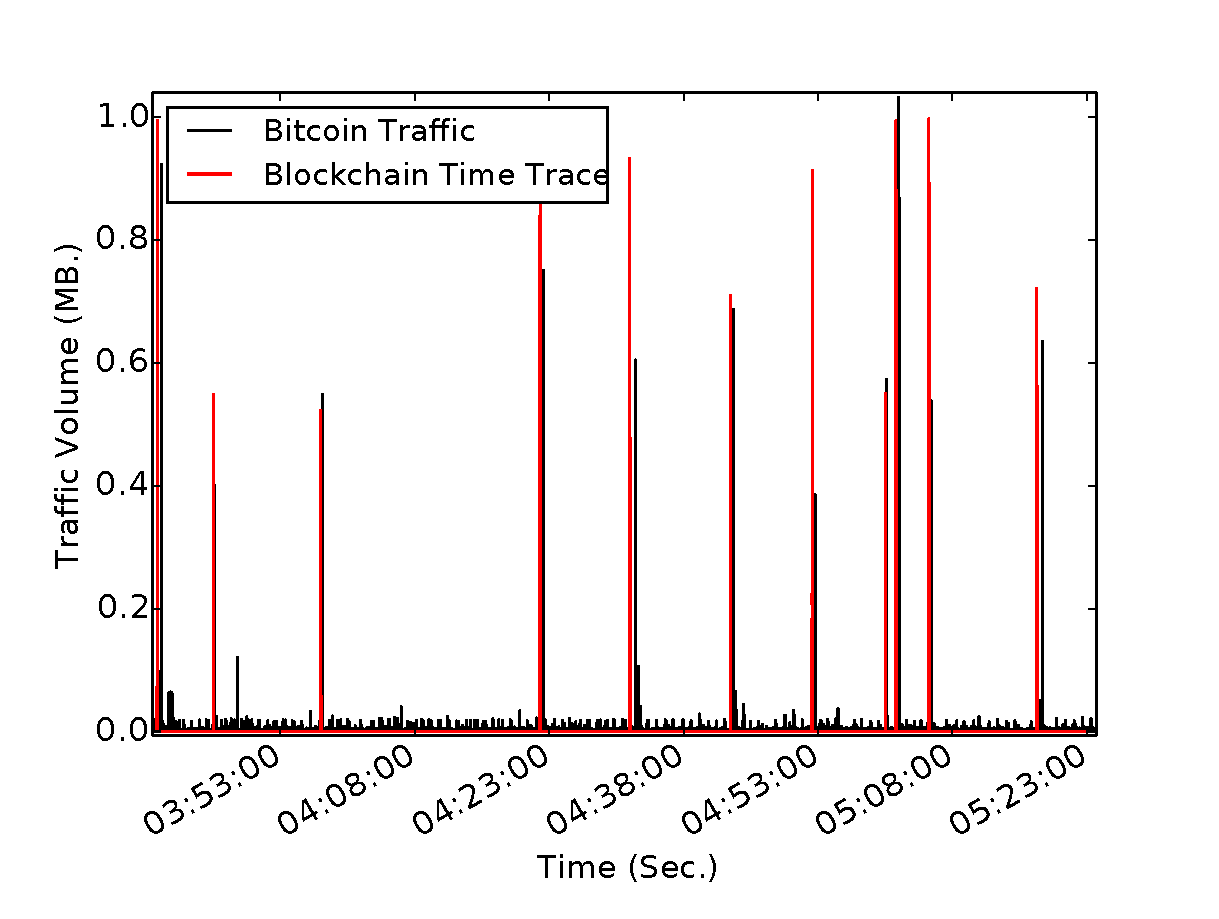
\includegraphics[width=\linewidth]{image/bitcoin_traffic_pattern.pdf}
\caption{Full block}
\label{fig:bitcoin_traffic_pattern}
\end{subfigure}
\centering
\begin{subfigure}{.48\linewidth}
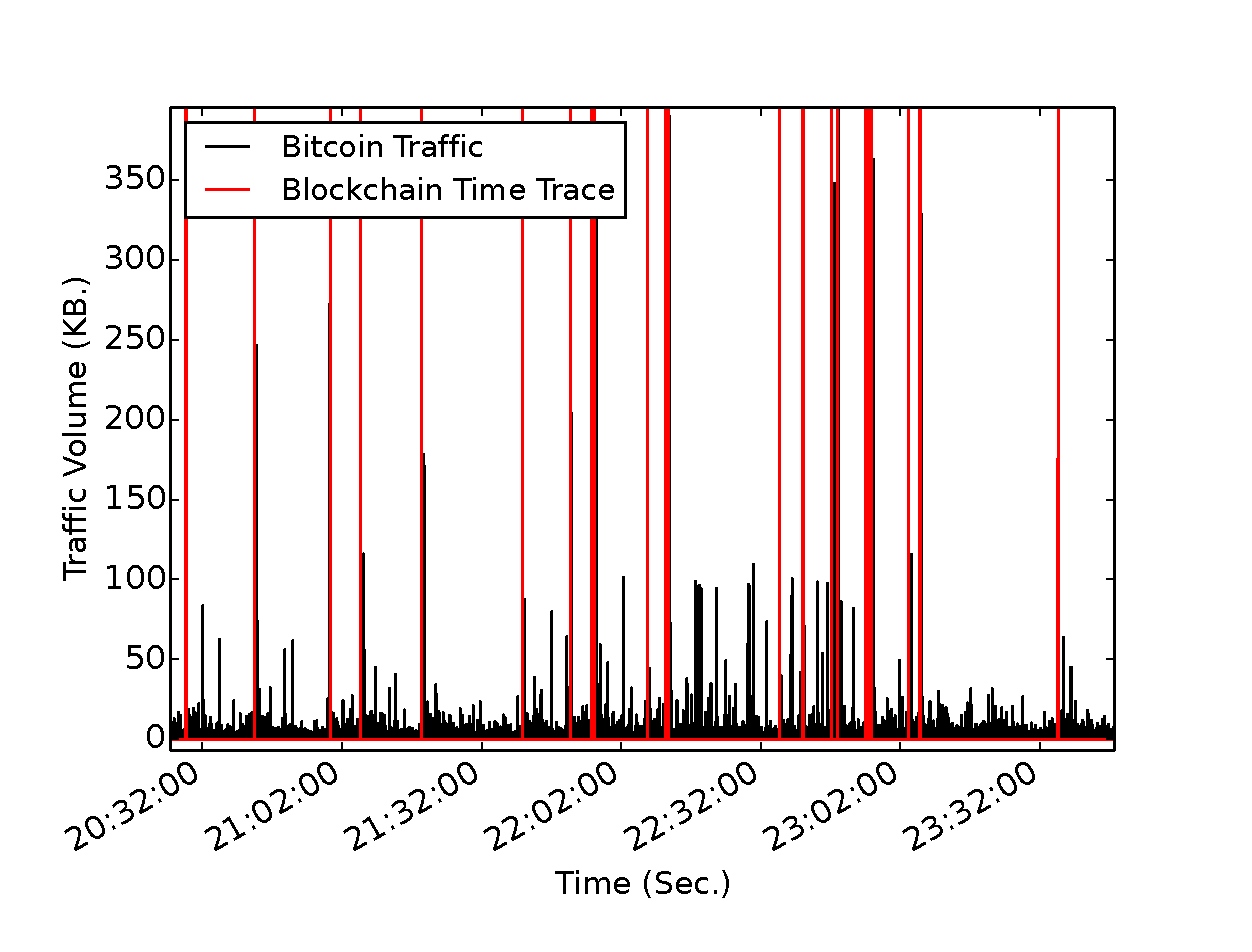
\includegraphics[width=\linewidth]{image/cmpctblock_traffic_volume_good.eps}
\caption{Compact block}
\label{fig:cmpctblock_traffic_volume_detectable}
\end{subfigure}
\caption{Comparing time of each block receive with time of blocks in the block chain in a) Full block and b) Compact block modes}
\end{figure*}

%\Q{Not quite sure what this is , and why we need this. Maybe elaborate?}\A{So this figure is showing the volume of transactions which the receiving haven't had and will receive it by \code{blocktxn} message, since it will send to receiving node after sending the compact block it also may have impact on the traffic volume at the point that we are expecting a block. }
 We also measure the volume of transactions missing from an announced compact block (we do so based on the payload length of \code{blocktxn} messages).
As described earlier,  a \bc client operating in the compact block mode will download such missing transactions.
%We measure the missing transactions based on the the payload length of \code{blocktxn} messages in the same way we measure the compact block sizes. 
This is shown in Figure~\ref{fig:blocktxn_volume}. 
As we can see most of the transactions have volumes less than 100 KB. 

 \begin{figure*}[!t]
\begin{subfigure}{.48\linewidth}
\centering
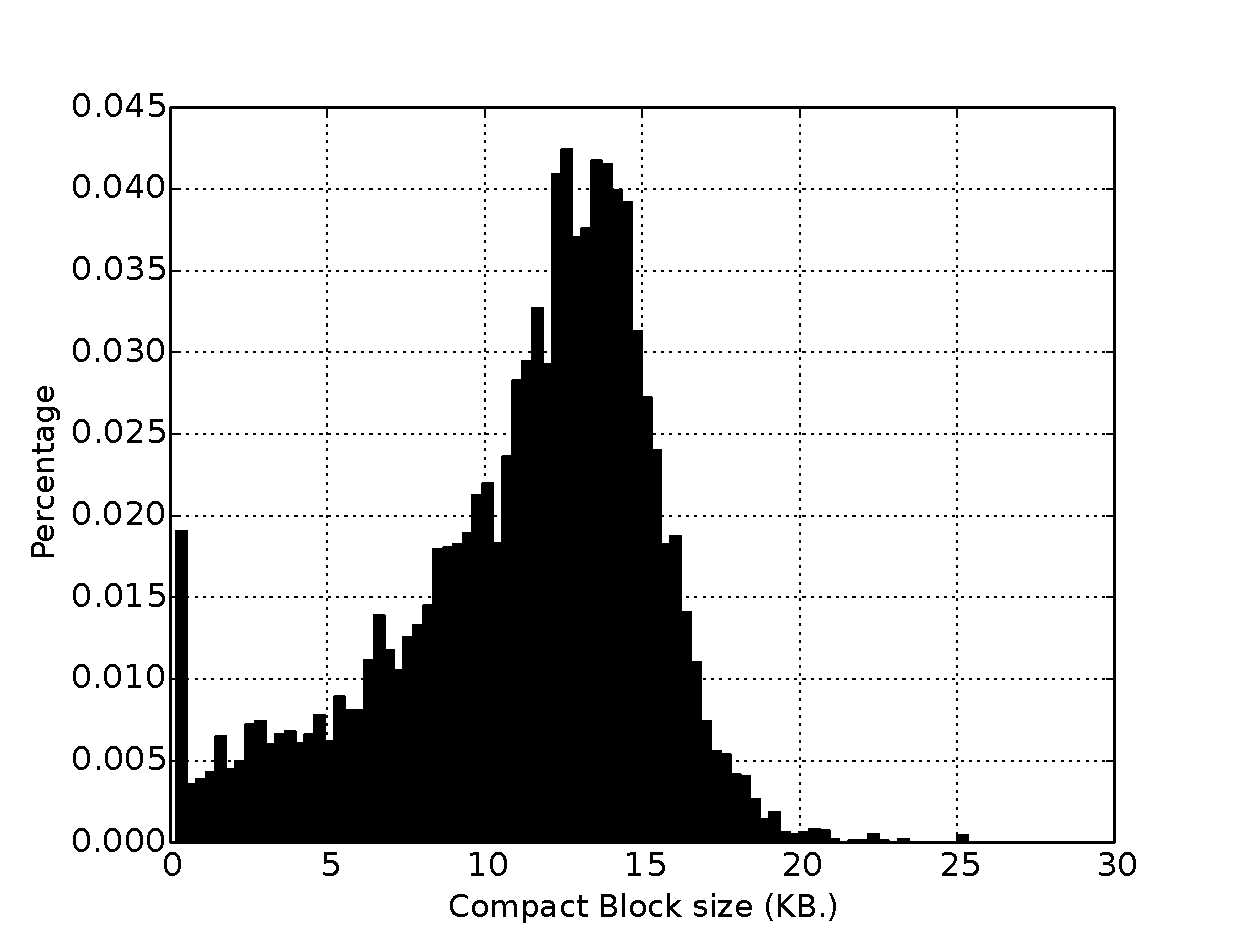
\includegraphics[width=\linewidth]{image/cmpctblock_traffic_volume.eps}
\caption{Histogram of the size of compact blocks}
\label{fig:cmpctblock_traffic_volume}
\end{subfigure}
\centering
\begin{subfigure}{.48\linewidth}
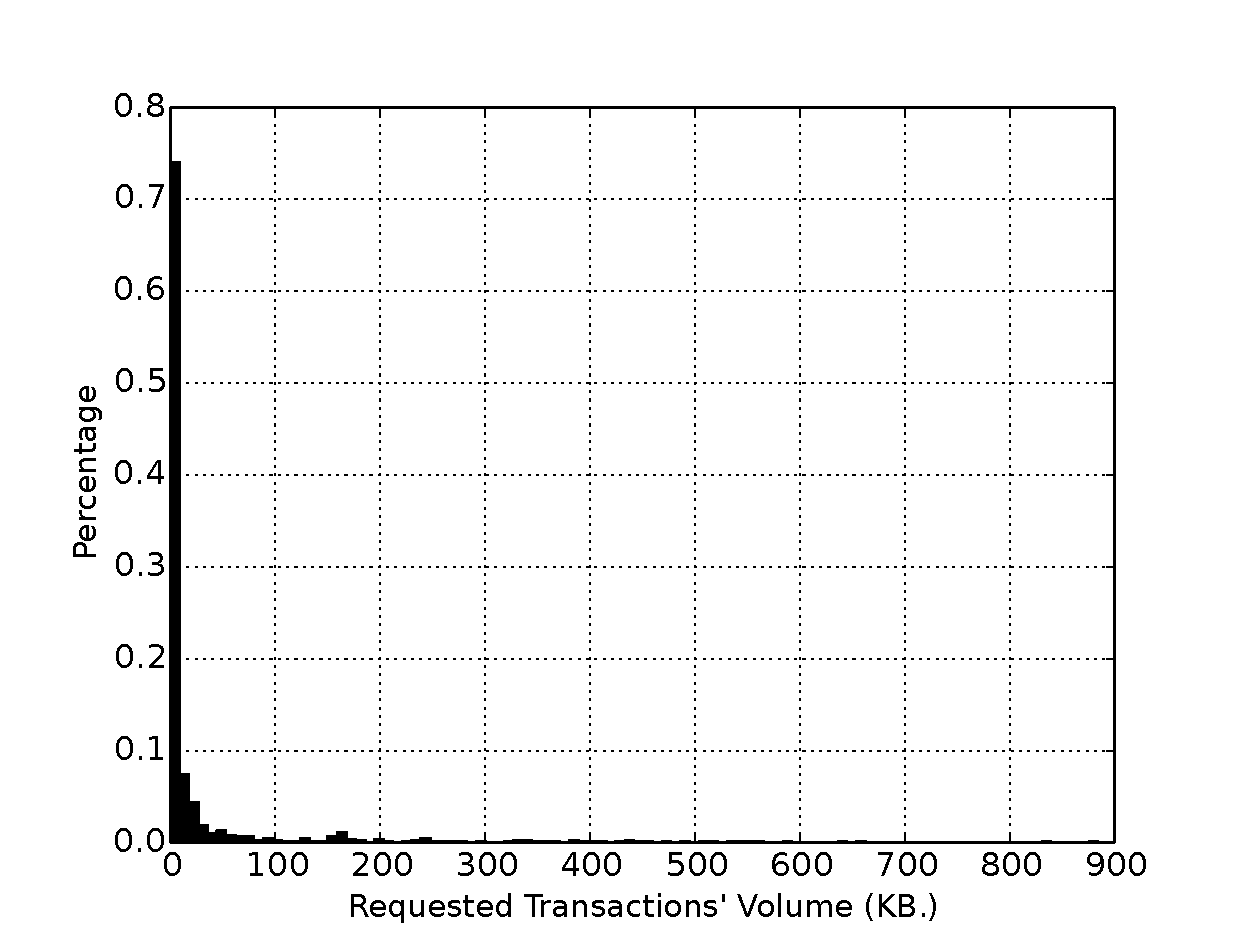
\includegraphics[width=\linewidth]{image/blocktxn_volume.eps}
\caption{Histogram of the size of missing transactions}
\label{fig:blocktxn_volume}
\end{subfigure}
\caption{Histogram of compact block mode components}
\label{fig:hist_cmp_component}
\end{figure*}

%The client's traffic shows a specific pattern, which makes us enable to come up with an algorithm to distinguish the Bitcoin traffic. We used our analysis in block propagation delay and Bitcoin traffic analysis to propose a correlation scheme. With the means of our correlation scheme we introduce a scheme to detect Bitcoin traffic.


%%%%%%%%%

\paragraphb{Block propagation latencies.} The propagation delay in the Bitcoin network is due to transmission delays and block verification by the receiving node at each hop. The transmission delay is the time to exchanging \textit{inv} and \textit{get data} messages, and sending the block via a \textit{block} message. 

 We measure block propagation delay by subtracting the receiving time of the block message and the time stamp in the header of the block message. Figures~\ref{fig:cmpctblock_time_difference} and \ref{fig:prop_delay} show the histogram of propagation delay for  $6000$ blocks in compact block and full block relaying, respectively. 
As shown in the figures, we can model this empirical data using a Beta distribution~\cite{probabilitybook}. %We choose a maximum for propagation delay such that $99\%$ of beta distribution is below that maximum. According to our measurements this value equals to $65$ seconds.\fatemeh{rewrite this part}

\begin{figure}[!t]% to have a bigger picture just add * at the end of figure
\begin{subfigure}{.48\linewidth}
\centering
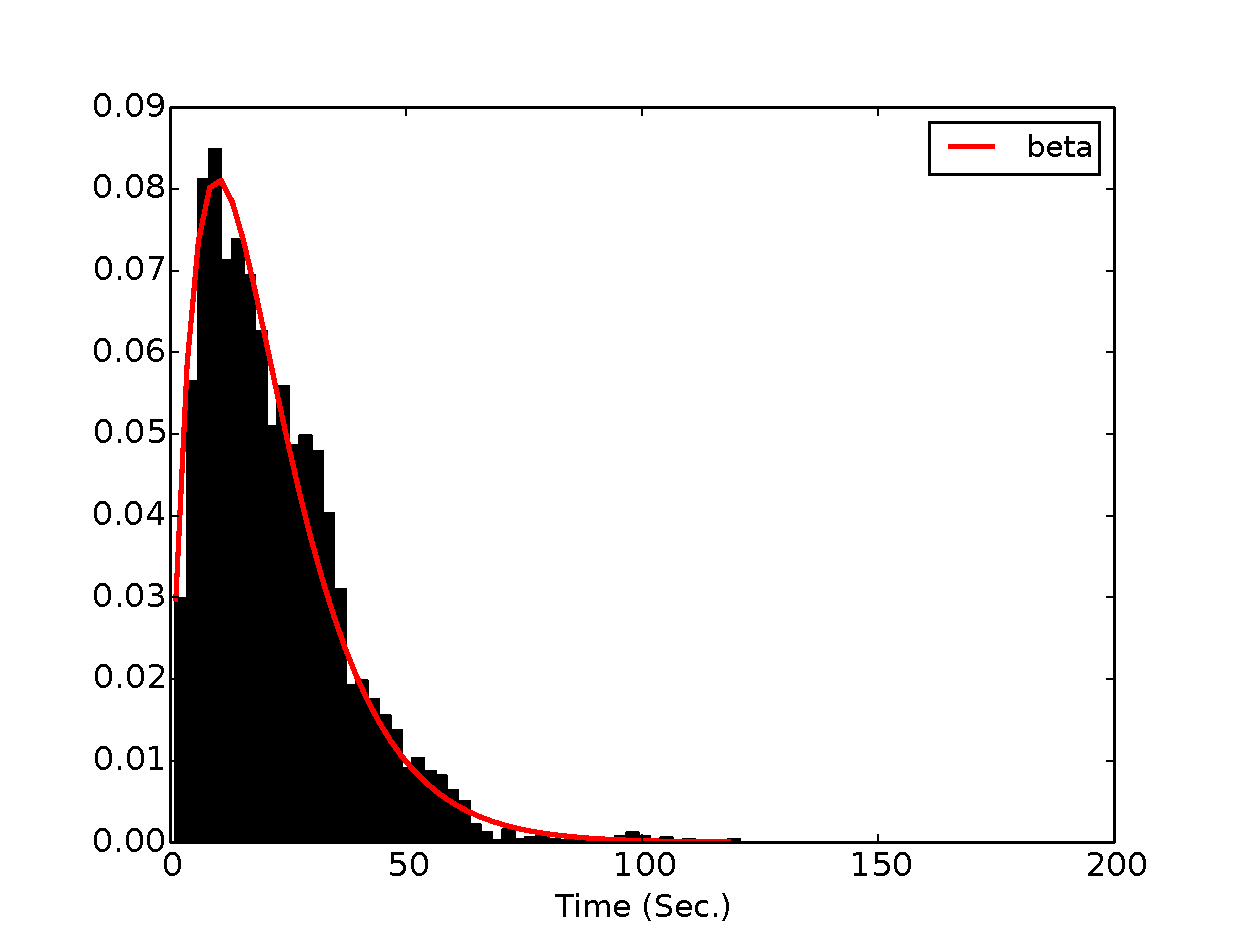
\includegraphics[width=\linewidth]{image/cmpctblock_time_difference.eps}
\caption{Compact block}
\label{fig:cmpctblock_time_difference}
\end{subfigure}
\centering
\begin{subfigure}{.48\linewidth}
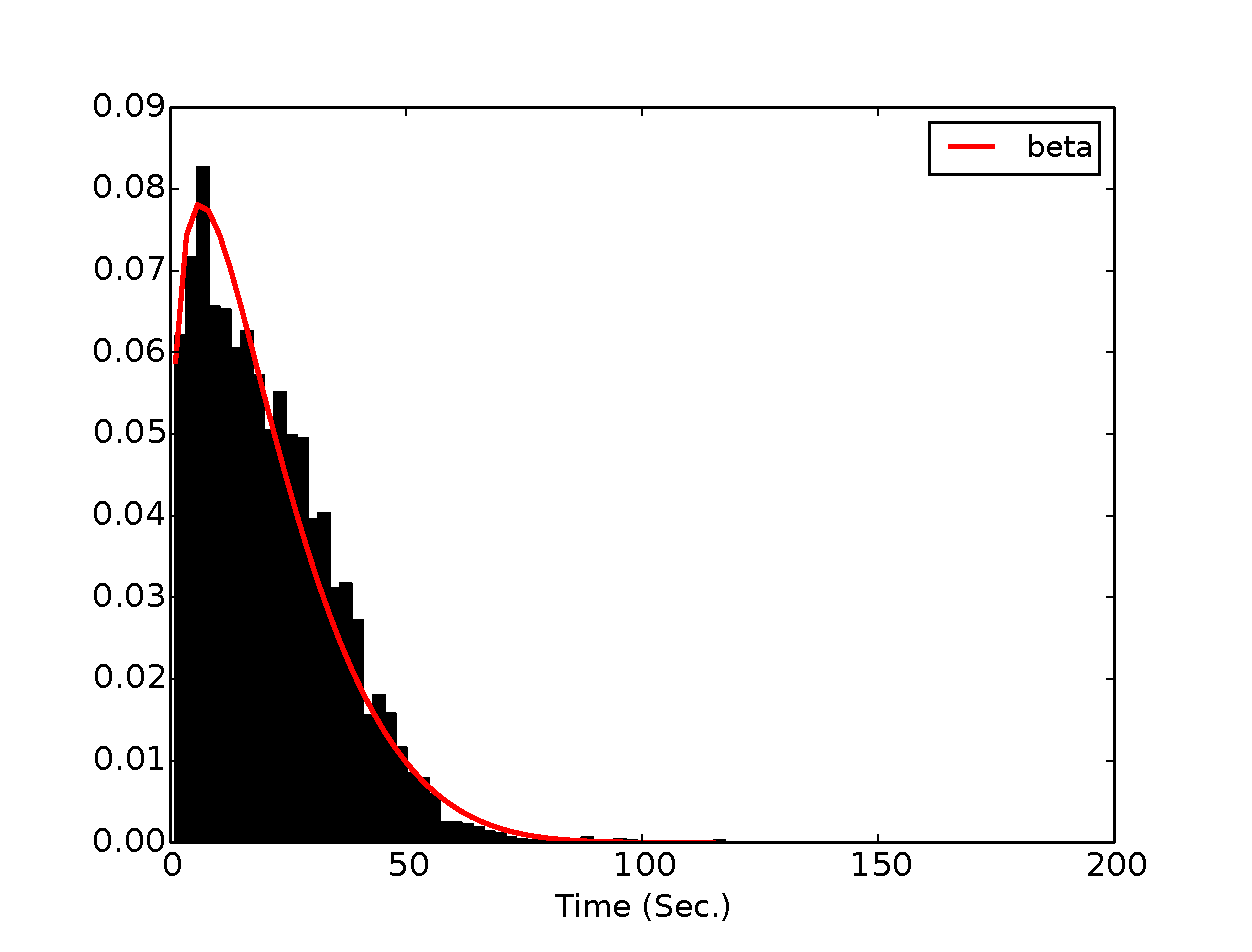
\includegraphics[width=\linewidth]{image/prop_delay_beta.eps}
\caption{Full block}
\label{fig:prop_delay}
\end{subfigure}
\caption{Histogram of block propagation delay}
\label{fig:prop_delay_full_compact}
\end{figure} 



%\paragraphb{Traffic patterns.} 
%In traditional block relaying, full block relaying, the client which its ledger is updated tries to download each block whenever they are announced to the client. Since at the time of writing this paper the block size is 1 MB, downloading full blocks causes a sudden burst in the traffic of network.
%
%\par Figure \ref{fig:bitcoin_traffic_pattern} shows the traffic of a client which is connected to Bitcoin network which relays full blocks. As we can see whenever we have a Bitcoin block in block-chain time trace there is a significant burst in the client traffic. 



%In the compact block relaying, since only a sketch of block is transmitted and there is no 1 MB bursts in the traffic, finding spikes would be harder. 



%%%%%%%%%%%%%%%%%%%%%%%%%%%%%%%%%%%%%%%%%%%%%%%%%%%%%%%%%%%
%%%%%%%%%%%%%%%%%%%%%%%%%%%%%%%%%%%%%%%%%%%%%%%%%%%%%%%%%%%
%%%%%%%%%%%%%%%%%%%%%%%%%%%%%%%%%%%%%%%%%%%%%%%%%%%%%%%%%%%